\documentclass[10pt,a4paper]{article}

\usepackage[margin=0.75cm]{geometry}
\usepackage[utf8]{inputenc}

\usepackage{amsmath}
\usepackage{amssymb}
\usepackage{biblatex}
\usepackage{textcomp}
\usepackage{gensymb}
\usepackage{paracol}
\usepackage{parskip}
\usepackage{tikz}
\usepackage{titlesec}
\usepackage{verbatim}
\usepackage{xcolor}

\titleformat{\section}[block]{\Large\bfseries\filcenter\color{black}}{\thesection}{1em}{}
\titleformat{\subsection}[block]{\bfseries\filcenter\color{black}}{\thesubsection}{1em}{}

\setlength{\columnsep}{25pt}

\tikzset{
    rounded-box/.style = {draw=cyan, fill=white, thin, rectangle, rounded corners, inner sep=5pt, inner ysep=10pt},
    rounded-box-title/.style = {fill=cyan, text=white, font=\bfseries},
}

\addbibresource{references.bib}

\begin{document}
\title{Calculus}

\section{Functions and Limits}

\subsection{Functions}

\begin{paracol}{2}

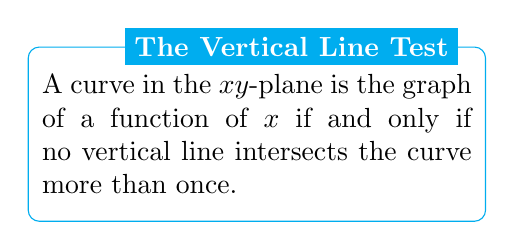
\begin{tikzpicture}
\node [rounded-box] (box){\begin{minipage}{0.45\textwidth}
    A curve in the $xy$-plane is the graph of a function of $x$ if and only if no vertical line intersects the curve more than once.
\end{minipage}};
\node[rounded-box-title, left=10pt] at (box.north east) {The Vertical Line Test};
\end{tikzpicture}

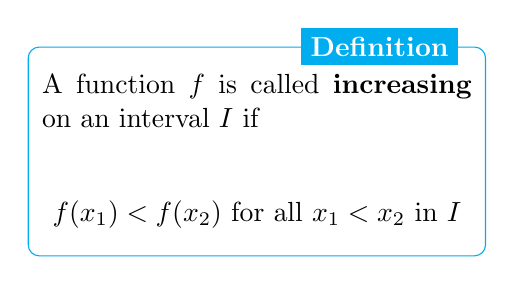
\begin{tikzpicture}
\node [rounded-box] (box){\begin{minipage}{0.45\textwidth}
    A function $f$ is called \textbf{increasing} on an interval $I$ if

    $$f(x_1) < f(x_2) \text{ for all } x_1 < x_2 \text{ in } I$$
\end{minipage}};
\node[rounded-box-title, left=10pt] at (box.north east) {Definition};
\end{tikzpicture}

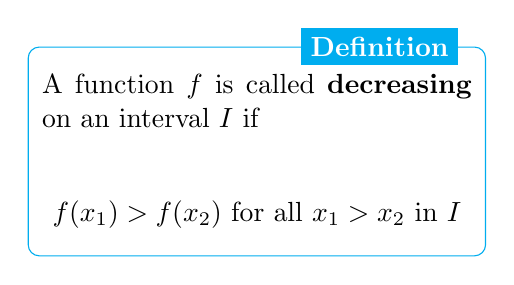
\begin{tikzpicture}
\node [rounded-box] (box){\begin{minipage}{0.45\textwidth}
    A function $f$ is called \textbf{decreasing} on an interval $I$ if

    $$f(x_1) > f(x_2) \text{ for all } x_1 > x_2 \text{ in } I$$
\end{minipage}};
\node[rounded-box-title, left=10pt] at (box.north east) {Definition};
\end{tikzpicture}

\switchcolumn

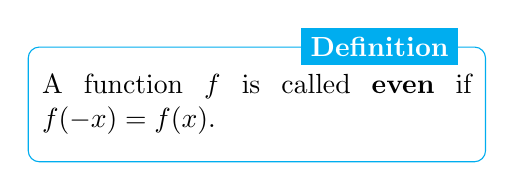
\begin{tikzpicture}
\node [rounded-box] (box){\begin{minipage}{0.45\textwidth}
    A function $f$ is called \textbf{even} if $f(-x) = f(x)$.
\end{minipage}};
\node[rounded-box-title, left=10pt] at (box.north east) {Definition};
\end{tikzpicture}

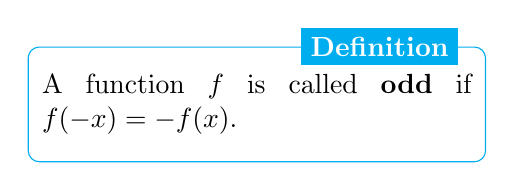
\begin{tikzpicture}
\node [rounded-box] (box){\begin{minipage}{0.45\textwidth}
    A function $f$ is called \textbf{odd} if $f(-x) = -f(x)$.
\end{minipage}};
\node[rounded-box-title, left=10pt] at (box.north east) {Definition};
\end{tikzpicture}

\begin{figure}
    \centering
    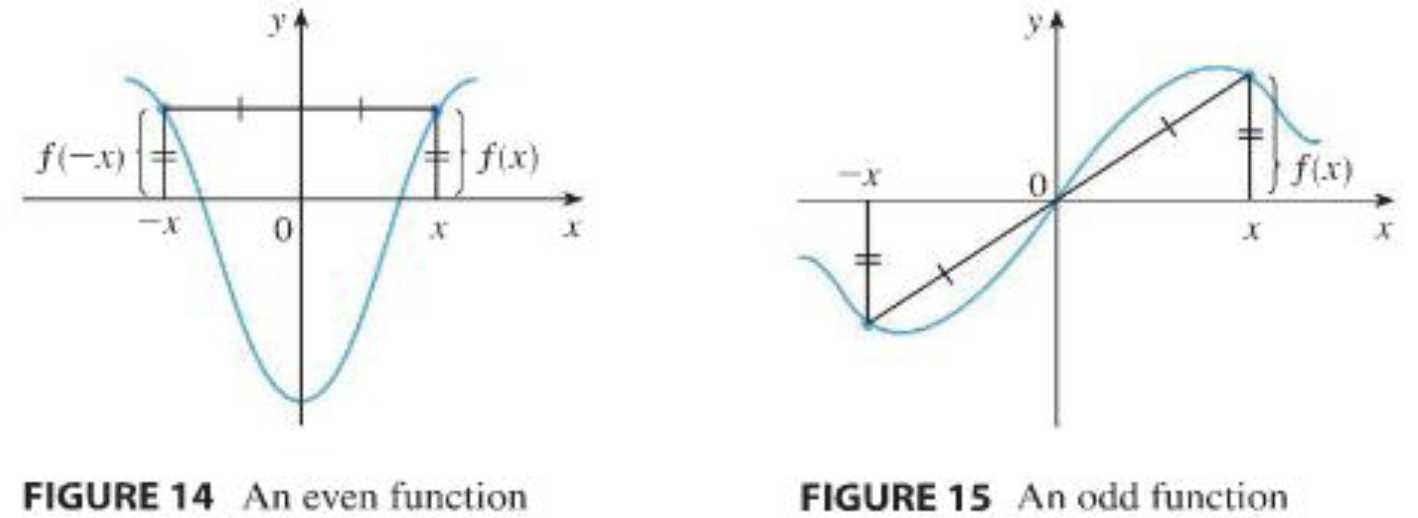
\includegraphics[width=0.95\linewidth]{even-odd-functions.png}
\end{figure}

\switchcolumn

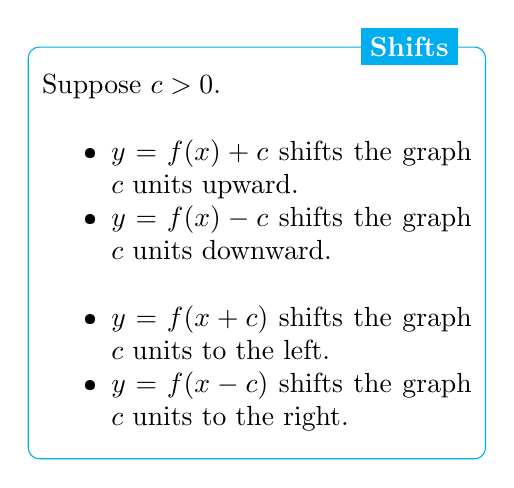
\begin{tikzpicture}
\node [rounded-box] (box){\begin{minipage}{0.45\textwidth}
    Suppose $c > 0$. \\

    \begin{itemize}
        \item $y = f(x) + c$ shifts the graph $c$ units upward.
        \item $y = f(x) - c$ shifts the graph $c$ units downward. \\

        \item $y = f(x + c)$ shifts the graph $c$ units to the left.
        \item $y = f(x - c)$ shifts the graph $c$ units to the right.
    \end{itemize}
\end{minipage}};
\node[rounded-box-title, left=10pt] at (box.north east) {Shifts};
\end{tikzpicture}

\switchcolumn

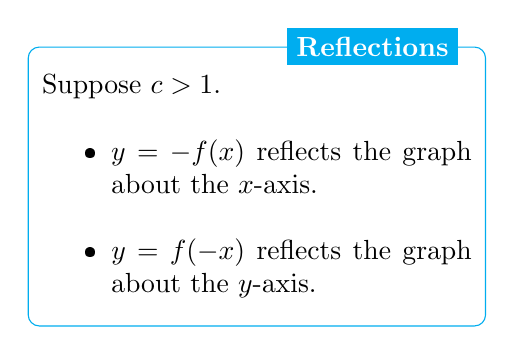
\begin{tikzpicture}
\node [rounded-box] (box){\begin{minipage}{0.45\textwidth}
    Suppose $c > 1$. \\

    \begin{itemize}
        \item $y = - f(x)$ reflects the graph about the $x$-axis. \\

        \item $y = f(-x)$ reflects the graph about the $y$-axis.
    \end{itemize}
\end{minipage}};
\node[rounded-box-title, left=10pt] at (box.north east) {Reflections};
\end{tikzpicture}

\switchcolumn

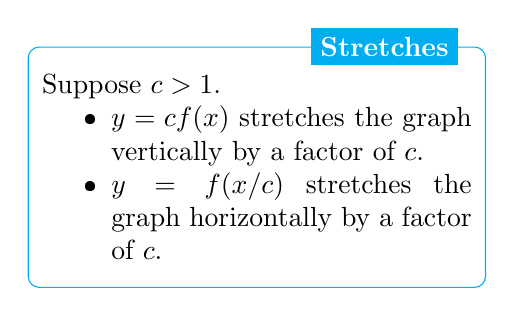
\begin{tikzpicture}
\node [rounded-box] (box){\begin{minipage}{0.45\textwidth}
    Suppose $c > 1$.

    \begin{itemize}
        \item $y = c f(x)$ stretches the graph vertically by a factor of $c$.

        \item $y = f(x / c)$ stretches the graph horizontally by a factor of $c$.
    \end{itemize}
\end{minipage}};
\node[rounded-box-title, left=10pt] at (box.north east) {Stretches};
\end{tikzpicture}

\switchcolumn

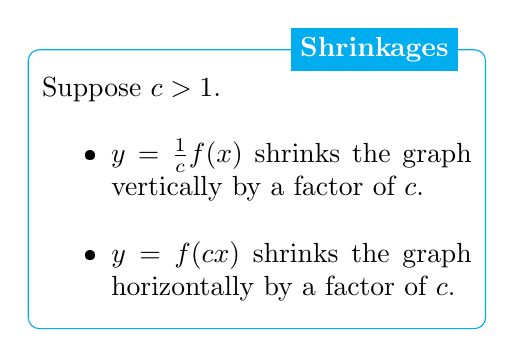
\begin{tikzpicture}
\node [rounded-box] (box){\begin{minipage}{0.45\textwidth}
    Suppose $c > 1$. \\

    \begin{itemize}
        \item $y = \frac{1}{c} f(x)$ shrinks the graph vertically by a factor of $c$. \\

        \item $y = f(c x)$ shrinks the graph horizontally by a factor of $c$.
    \end{itemize}
\end{minipage}};
\node[rounded-box-title, left=10pt] at (box.north east) {Shrinkages};
\end{tikzpicture}

\end{paracol}

\subsection{Limits}

\begin{paracol}{2}

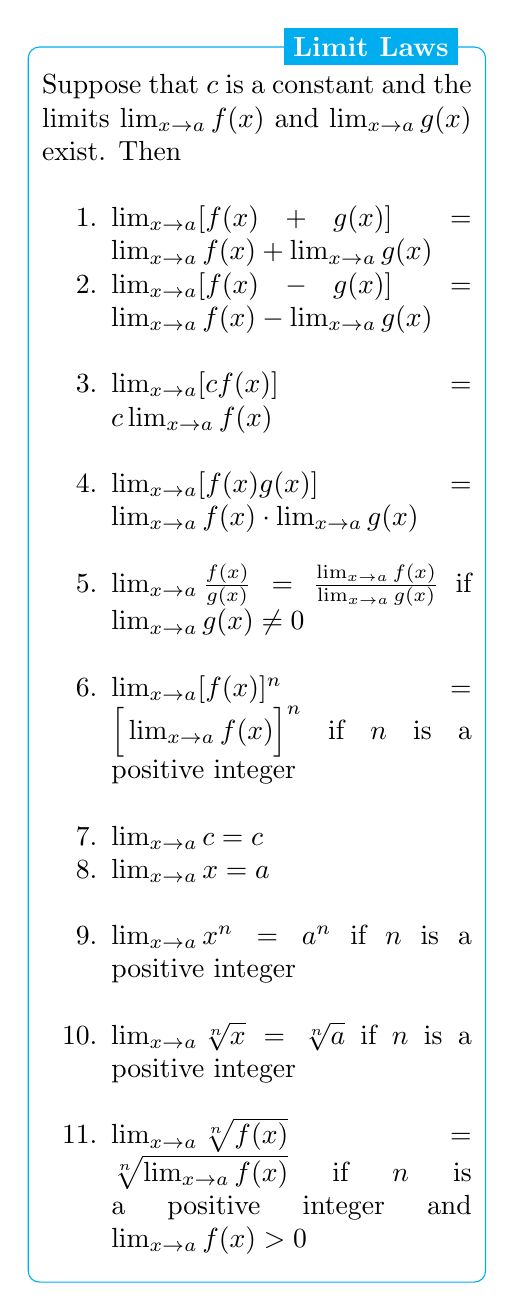
\begin{tikzpicture}
\node [rounded-box] (box){\begin{minipage}{0.45\textwidth}
    Suppose that $c$ is a constant and the limits $\lim_{x \rightarrow a} f(x)$ and $\lim_{x \rightarrow a} g(x)$ exist. Then \\

    \begin{enumerate}
        \item $\lim_{x \rightarrow a} [f(x) + g(x)] = \lim_{x \rightarrow a} f(x) + \lim_{x \rightarrow a} g(x)$

        \item $\lim_{x \rightarrow a} [f(x) - g(x)] = \lim_{x \rightarrow a} f(x) - \lim_{x \rightarrow a} g(x)$ \\

        \item $\lim_{x \rightarrow a} [c f(x)] = c \lim_{x \rightarrow a} f(x)$ \\

        \item $\lim_{x \rightarrow a} [f(x) g(x)] = \lim_{x \rightarrow a} f(x) \cdot \lim_{x \rightarrow a} g(x)$ \\

        \item $\lim_{x \rightarrow a} \frac{f(x)}{g(x)} = \frac{\lim_{x \rightarrow a} f(x)}{\lim_{x \rightarrow a} g(x)}$ if $\lim_{x \rightarrow a} g(x) \neq 0$ \\

        \item $\lim_{x \rightarrow a} [f(x)]^n = \Big[ \lim_{x \rightarrow a} f(x) \Big]^n$ if $n$ is a positive integer \\

        \item $\lim_{x \rightarrow a} c = c$

        \item $\lim_{x \rightarrow a} x = a$ \\

        \item $\lim_{x \rightarrow a} x^n = a^n$ if $n$ is a positive integer \\

        \item $\lim_{x \rightarrow a} \sqrt[n]{x} = \sqrt[n]{a}$ if $n$ is a positive integer \\

        \item $\lim_{x \rightarrow a} \sqrt[n]{f(x)} = \sqrt[n]{\lim_{x \rightarrow a} f(x)}$ if $n$ is a positive integer and $\lim_{x \rightarrow a} f(x) > 0$
    \end{enumerate}
\end{minipage}};
\node[rounded-box-title, left=10pt] at (box.north east) {Limit Laws};
\end{tikzpicture}

\switchcolumn

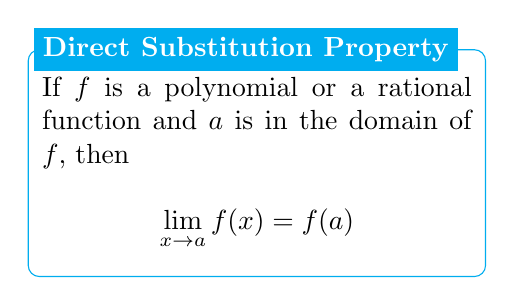
\begin{tikzpicture}
\node [rounded-box] (box){\begin{minipage}{0.45\textwidth}
    If $f$ is a polynomial or a rational function and $a$ is in the domain of $f$, then

    $$\lim_{x \rightarrow a} f(x) = f(a)$$
\end{minipage}};
\node[rounded-box-title, left=10pt] at (box.north east) {Direct Substitution Property};
\end{tikzpicture}

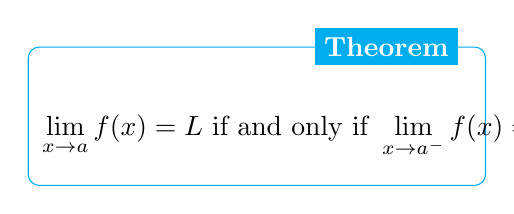
\begin{tikzpicture}
\node [rounded-box] (box){\begin{minipage}{0.45\textwidth}
    $$\lim_{x \rightarrow a} f(x) = L \text{ if and only if } \lim_{x \rightarrow a^-} f(x) = \lim_{x \rightarrow a^+} f(x) = L$$
\end{minipage}};
\node[rounded-box-title, left=10pt] at (box.north east) {Theorem};
\end{tikzpicture}

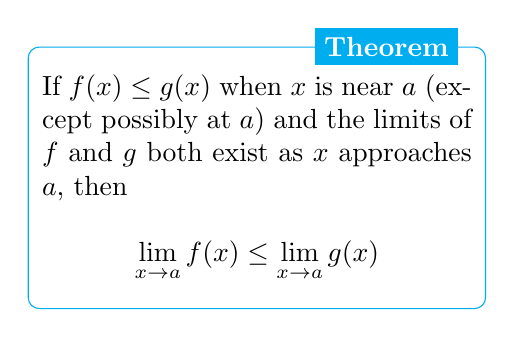
\begin{tikzpicture}
\node [rounded-box] (box){\begin{minipage}{0.45\textwidth}
    If $f(x) \leq g(x)$ when $x$ is near $a$ (except possibly at $a$) and the limits of $f$ and $g$ both exist as $x$ approaches $a$, then

    $$\lim_{x \rightarrow a} f(x) \leq \lim_{x \rightarrow a} g(x)$$
\end{minipage}};
\node[rounded-box-title, left=10pt] at (box.north east) {Theorem};
\end{tikzpicture}

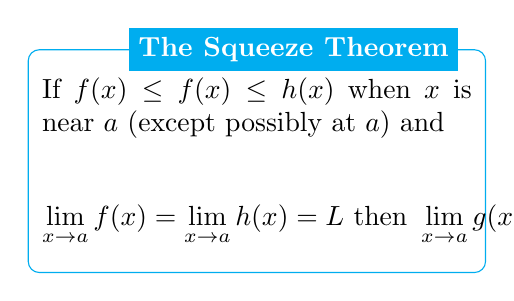
\begin{tikzpicture}
\node [rounded-box] (box){\begin{minipage}{0.45\textwidth}
    If $f(x) \leq f(x) \leq h(x)$ when $x$ is near $a$ (except possibly at $a$) and

    $$\lim_{x \rightarrow a} f(x) = \lim_{x \rightarrow a} h(x) = L \text{ then } \lim_{x \rightarrow a} g(x) = L$$
\end{minipage}};
\node[rounded-box-title, left=10pt] at (box.north east) {The Squeeze Theorem};
\end{tikzpicture}

\end{paracol}

\subsection{Continuity}

\begin{paracol}{2}

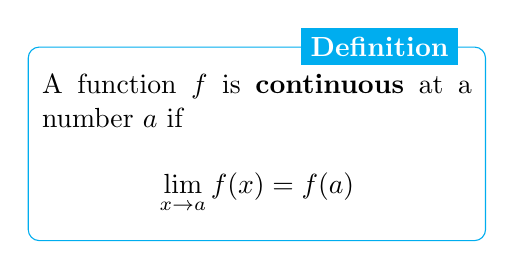
\begin{tikzpicture}
\node [rounded-box] (box){\begin{minipage}{0.45\textwidth}
    A function $f$ is \textbf{continuous} at a number $a$ if

    $$\lim_{x \rightarrow a} f(x) = f(a)$$
\end{minipage}};
\node[rounded-box-title, left=10pt] at (box.north east) {Definition};
\end{tikzpicture}

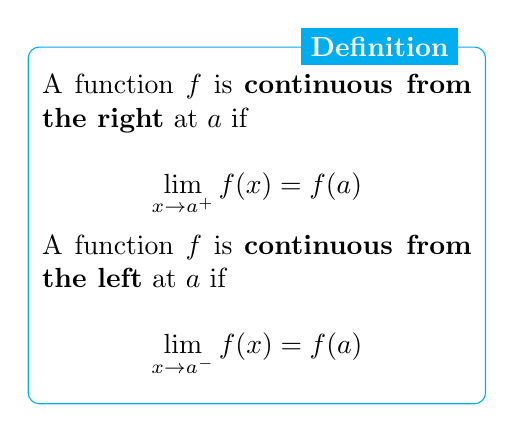
\begin{tikzpicture}
\node [rounded-box] (box){\begin{minipage}{0.45\textwidth}
    A function $f$ is \textbf{continuous from the right} at $a$ if

    $$\lim_{x \rightarrow a^+} f(x) = f(a)$$

    A function $f$ is \textbf{continuous from the left} at $a$ if

    $$\lim_{x \rightarrow a^-} f(x) = f(a)$$
\end{minipage}};
\node[rounded-box-title, left=10pt] at (box.north east) {Definition};
\end{tikzpicture}

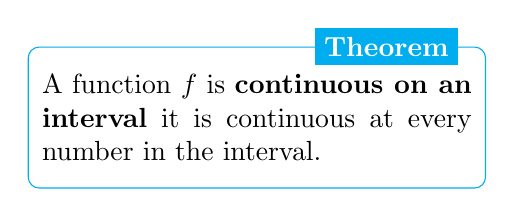
\begin{tikzpicture}
\node [rounded-box] (box){\begin{minipage}{0.45\textwidth}
    A function $f$ is \textbf{continuous on an interval} it is continuous at every number in the interval.
\end{minipage}};
\node[rounded-box-title, left=10pt] at (box.north east) {Theorem};
\end{tikzpicture}

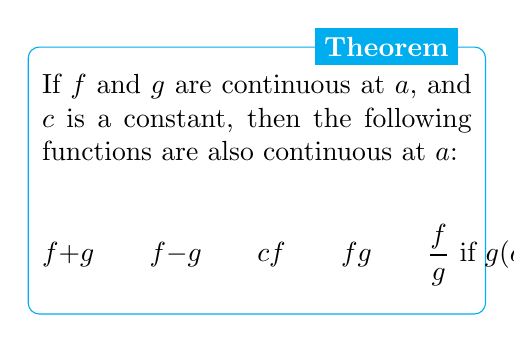
\begin{tikzpicture}
\node [rounded-box] (box){\begin{minipage}{0.45\textwidth}
    If $f$ and $g$ are continuous at $a$, and $c$ is a constant, then the following functions are also continuous at $a$:

    $$f + g \qquad f - g \qquad cf \qquad fg \qquad \frac{f}{g} \text{ if } g(a) \neq 0$$
\end{minipage}};
\node[rounded-box-title, left=10pt] at (box.north east) {Theorem};
\end{tikzpicture}

\switchcolumn

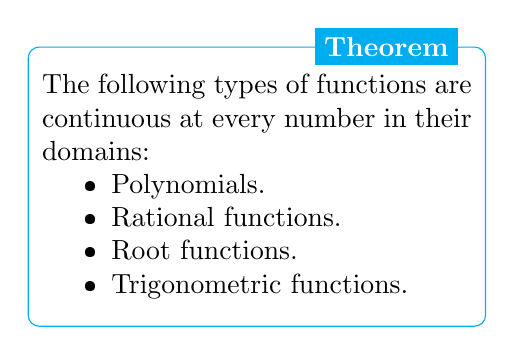
\begin{tikzpicture}
\node [rounded-box] (box){\begin{minipage}{0.45\textwidth}
    The following types of functions are continuous at every number in their domains:

    \begin{itemize}
        \item Polynomials.
        \item Rational functions.
        \item Root functions.
        \item Trigonometric functions.
    \end{itemize}
\end{minipage}};
\node[rounded-box-title, left=10pt] at (box.north east) {Theorem};
\end{tikzpicture}

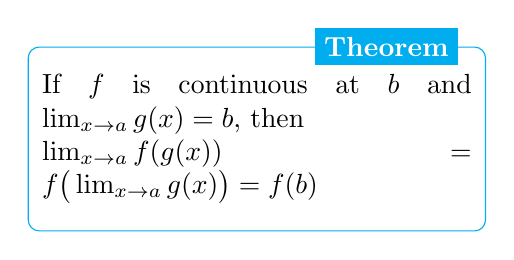
\begin{tikzpicture}
\node [rounded-box] (box){\begin{minipage}{0.45\textwidth}
    If $f$ is continuous at $b$ and $\lim_{x \rightarrow a} g(x) = b$, then

    $\lim_{x \rightarrow a} f(g(x)) = f\big( \lim_{x \rightarrow a} g(x) \big) = f(b)$
\end{minipage}};
\node[rounded-box-title, left=10pt] at (box.north east) {Theorem};
\end{tikzpicture}

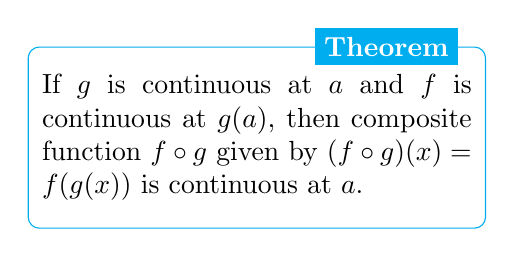
\begin{tikzpicture}
\node [rounded-box] (box){\begin{minipage}{0.45\textwidth}
    If $g$ is continuous at $a$ and $f$ is continuous at $g(a)$, then composite function $f \circ g$ given by $(f \circ g)(x) = f(g(x))$ is continuous at $a$.
\end{minipage}};
\node[rounded-box-title, left=10pt] at (box.north east) {Theorem};
\end{tikzpicture}

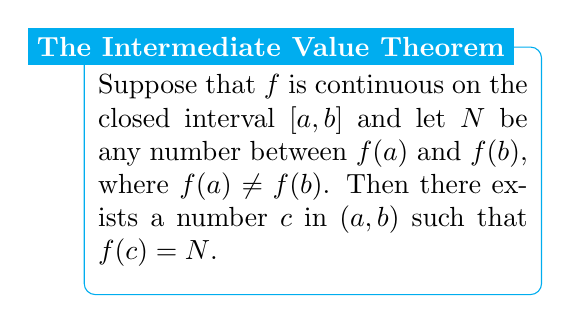
\begin{tikzpicture}
\node [rounded-box] (box){\begin{minipage}{0.45\textwidth}
    Suppose that $f$ is continuous on the closed interval $[a, b]$ and let $N$ be any number between $f(a)$ and $f(b)$, where $f(a) \neq f(b)$. Then there exists a number $c$ in $(a, b)$ such that $f(c) = N$.
\end{minipage}};
\node[rounded-box-title, left=10pt] at (box.north east) {The Intermediate Value Theorem};
\end{tikzpicture}

That is, a continuous function takes on every intermediate value between the function values $f(a)$ and $f(b)$ at least once.

\end{paracol}

\subsection{Inverse Functions}

\begin{paracol}{2}

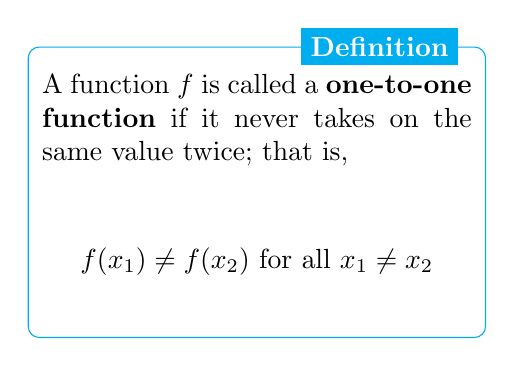
\begin{tikzpicture}
\node [rounded-box] (box){\begin{minipage}{0.45\textwidth}
    A function $f$ is called a \textbf{one-to-one function} if it never takes on the same value twice; that is,

    \vspace{5pt}

    $$f(x_1) \neq f(x_2) \text{ for all } x_1 \neq x_2$$

    \vspace{2.5pt}
\end{minipage}};
\node[rounded-box-title, left=10pt] at (box.north east) {Definition};
\end{tikzpicture}

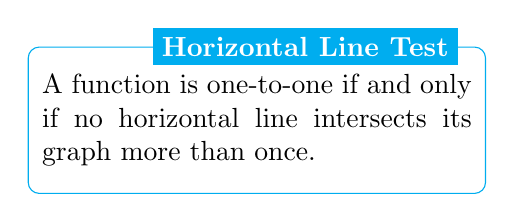
\begin{tikzpicture}
\node [rounded-box] (box){\begin{minipage}{0.45\textwidth}
    A function is one-to-one if and only if no horizontal line intersects its graph more than once.
\end{minipage}};
\node[rounded-box-title, left=10pt] at (box.north east) {Horizontal Line Test};
\end{tikzpicture}

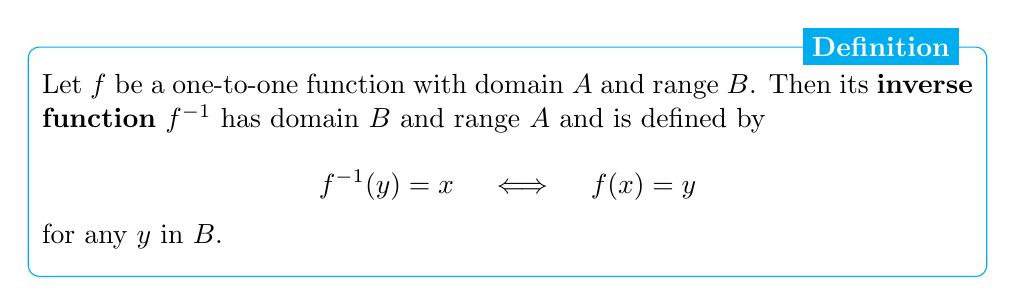
\begin{tikzpicture}
\node [rounded-box] (box){\begin{minipage}{0.975\textwidth}
    Let $f$ be a one-to-one function with domain $A$ and range $B$. Then its \textbf{inverse function} $f^{-1}$ has domain $B$ and range $A$ and is defined by

    $$f^{-1}(y) = x \quad \iff \quad f(x) = y$$

    for any $y$ in $B$.
\end{minipage}};
\node[rounded-box-title, left=10pt] at (box.north east) {Definition};
\end{tikzpicture}

\switchcolumn

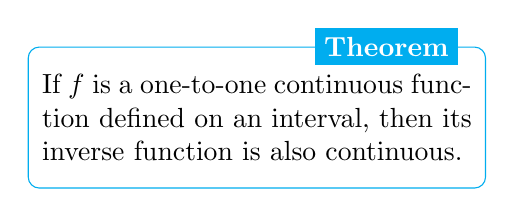
\begin{tikzpicture}
\node [rounded-box] (box){\begin{minipage}{0.45\textwidth}
    If $f$ is a one-to-one continuous function defined on an interval, then its inverse function is also continuous.
\end{minipage}};
\node[rounded-box-title, left=10pt] at (box.north east) {Theorem};
\end{tikzpicture}

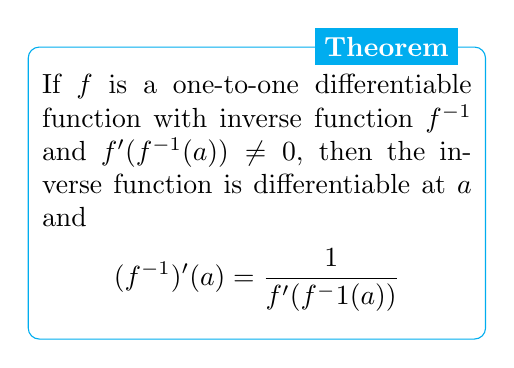
\begin{tikzpicture}
\node [rounded-box] (box){\begin{minipage}{0.45\textwidth}
    If $f$ is a one-to-one differentiable function with inverse function $f^{-1}$ and $f'(f^{-1}(a)) \neq 0$, then the inverse function is differentiable at $a$ and

    \vspace{-5pt}

    $$(f^{-1})'(a) = \frac{1}{f'(f^-1(a))}$$
\end{minipage}};
\node[rounded-box-title, left=10pt] at (box.north east) {Theorem};
\end{tikzpicture}

\end{paracol}

\subsection{Asymptotes}

\begin{paracol}{2}

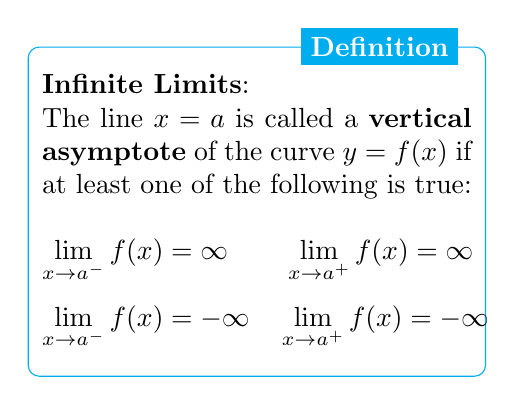
\begin{tikzpicture}
\node [rounded-box] (box){\begin{minipage}{0.45\textwidth}
    \textbf{Infinite Limits}:
    
    The line $x = a$ is called a \textbf{vertical asymptote} of the curve $y = f(x)$ if at least one of the following is true:

    \vspace{-10pt}

    $$\lim_{x \rightarrow a^-} f(x) = \infty \qquad \lim_{x \rightarrow a^+} f(x) = \infty \qquad \lim_{x \rightarrow a} f(x) = \infty$$

    \vspace{-20pt}

    $$\lim_{x \rightarrow a^-} f(x) = -\infty \quad \lim_{x \rightarrow a^+} f(x) = -\infty \quad \lim_{x \rightarrow a} f(x) = -\infty$$
\end{minipage}};
\node[rounded-box-title, left=10pt] at (box.north east) {Definition};
\end{tikzpicture}

\switchcolumn

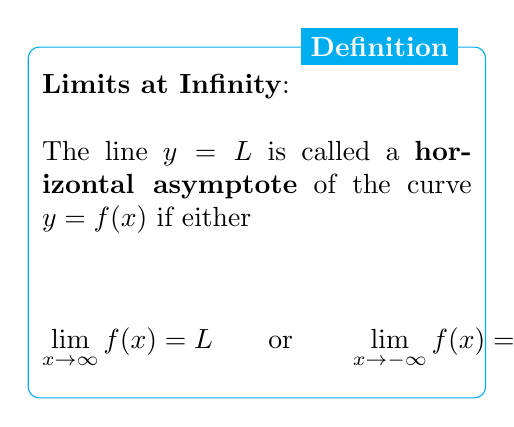
\begin{tikzpicture}
\node [rounded-box] (box){\begin{minipage}{0.45\textwidth}
    \textbf{Limits at Infinity}: \\
    
    The line $y = L$ is called a \textbf{horizontal asymptote} of the curve $y = f(x)$ if either

    \vspace{10pt}

    $$\lim_{x \rightarrow \infty} f(x) = L \qquad \text{or} \qquad \lim_{x \rightarrow -\infty} f(x) = L$$
\end{minipage}};
\node[rounded-box-title, left=10pt] at (box.north east) {Definition};
\end{tikzpicture}

\end{paracol}

The line $y = mx + b$ is called a \textbf{slant asymptote} if $\lim_{x \rightarrow \pm \infty} f(x) - (mx + b) = 0$.

\subsection{Indeterminate Forms and l'Hospital's Rule}

\begin{paracol}{2}

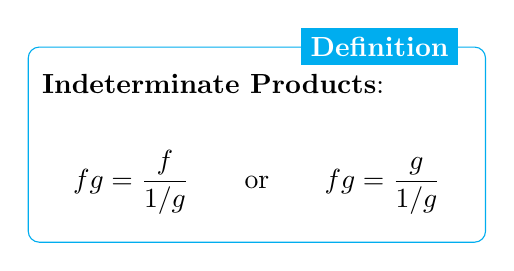
\begin{tikzpicture}
\node [rounded-box] (box){\begin{minipage}{0.45\textwidth}
    \textbf{Indeterminate Products}:

    \vspace{-2.5pt}

    $$fg = \frac{f}{1 / g} \qquad \text{or} \qquad fg = \frac{g}{1 / g}$$
\end{minipage}};
\node[rounded-box-title, left=10pt] at (box.north east) {Definition};
\end{tikzpicture}

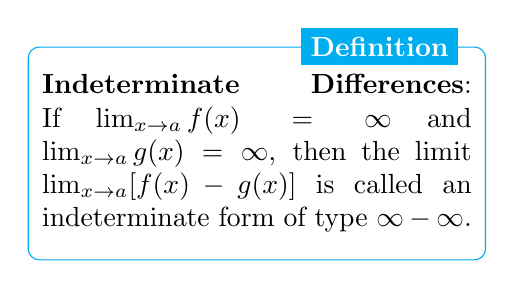
\begin{tikzpicture}
\node [rounded-box] (box){\begin{minipage}{0.45\textwidth}
    \textbf{Indeterminate Differences}: If $\lim_{x \rightarrow a} f(x) = \infty$ and $\lim_{x \rightarrow a} g(x) = \infty$, then the limit $\lim_{x \rightarrow a} [f(x) - g(x)]$ is called an indeterminate form of type $\infty - \infty$.
\end{minipage}};
\node[rounded-box-title, left=10pt] at (box.north east) {Definition};
\end{tikzpicture}

\switchcolumn

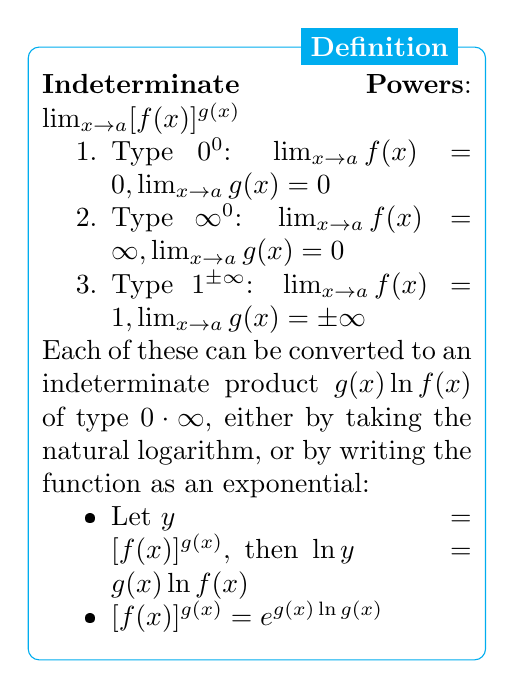
\begin{tikzpicture}
\node [rounded-box] (box){\begin{minipage}{0.45\textwidth}
    \textbf{Indeterminate Powers}: $\lim_{x \rightarrow a} [f(x)]^{g(x)}$

    \begin{enumerate}
        \item Type $0^0$: $\lim_{x \rightarrow a} f(x) = 0, \lim_{x \rightarrow a} g(x) = 0$
        \item Type $\infty^0$: $\lim_{x \rightarrow a} f(x) = \infty, \lim_{x \rightarrow a} g(x) = 0$
        \item Type $1^{\pm \infty}$: $\lim_{x \rightarrow a} f(x) = 1, \lim_{x \rightarrow a} g(x) = \pm \infty$
    \end{enumerate}

    Each of these can be converted to an indeterminate product $g(x) \ln{f(x)}$ of type $0 \cdot \infty$, either by taking the natural logarithm, or by writing the function as an exponential:

    \begin{itemize}
        \item $\text{Let } y = [f(x)]^{g(x)}, \text{ then } \ln{y} = g(x) \ln{f(x)}$
        \item $[f(x)]^{g(x)} = e^{g(x) \ln{g(x)}}$
    \end{itemize}
\end{minipage}};
\node[rounded-box-title, left=10pt] at (box.north east) {Definition};
\end{tikzpicture}

\end{paracol}

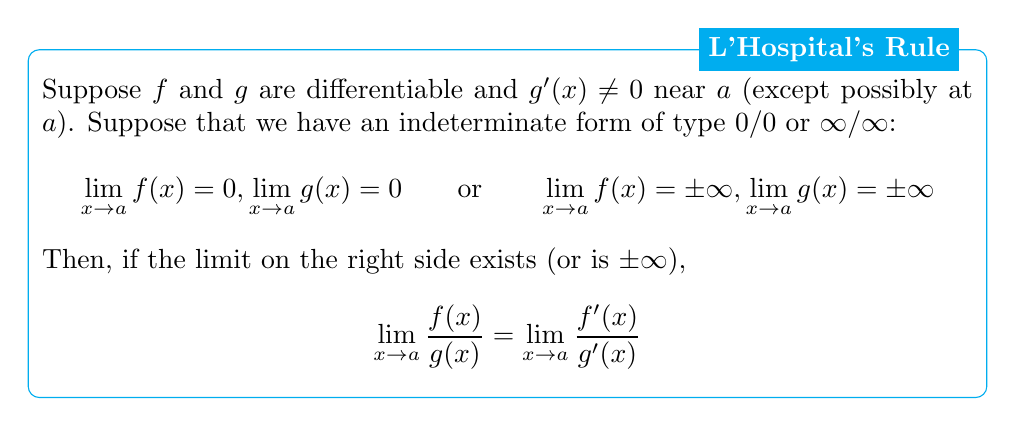
\begin{tikzpicture}
\node [rounded-box] (box){\begin{minipage}{0.975\textwidth}
    Suppose $f$ and $g$ are differentiable and $g'(x) \neq 0$ near $a$ (except possibly at $a$). Suppose that we have an indeterminate form of type $0/0$ or $\infty/\infty$:

    \vspace{-10pt}

    $$\lim_{x \rightarrow a} f(x) = 0,  \lim_{x \rightarrow a} g(x) = 0 \qquad \text{or} \qquad \lim_{x \rightarrow a} f(x) = \pm \infty, \lim_{x \rightarrow a} g(x) = \pm \infty$$

    Then, if the limit on the right side exists (or is $\pm \infty$),

    $$\lim_{x \rightarrow a} \frac{f(x)}{g(x)} = \lim_{x \rightarrow a} \frac{f'(x)}{g'(x)}$$
\end{minipage}};
\node[rounded-box-title, left=10pt] at (box.north east) {L'Hospital's Rule};
\end{tikzpicture}

\section{Differentiation}

\subsection{Derivatives and Rates of Change}

\begin{paracol}{2}

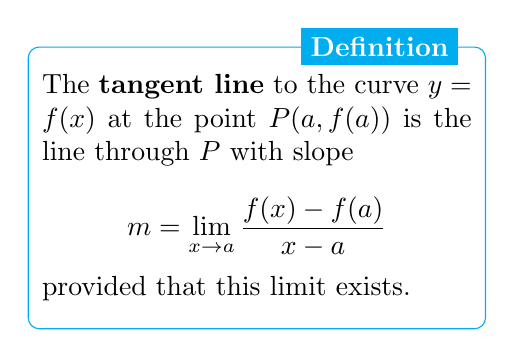
\begin{tikzpicture}
\node [rounded-box] (box){\begin{minipage}{0.45\textwidth}
    The \textbf{tangent line} to the curve $y = f(x)$ at the point $P(a, f(a))$ is the line through $P$ with slope

    $$m = \lim_{x \rightarrow a} \frac{f(x) - f(a)}{x - a}$$

    provided that this limit exists.
\end{minipage}};
\node[rounded-box-title, left=10pt] at (box.north east) {Definition};
\end{tikzpicture}

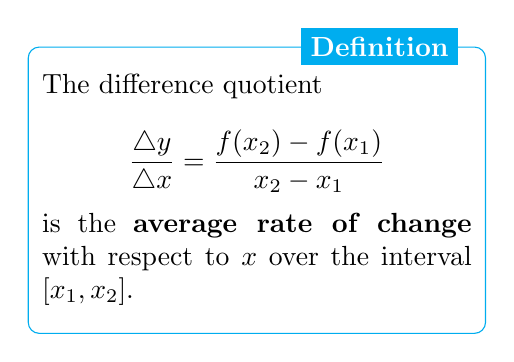
\begin{tikzpicture}
\node [rounded-box] (box){\begin{minipage}{0.45\textwidth}
    The difference quotient

    $$\frac{\triangle y}{\triangle x} = \frac{f(x_2) - f(x_1)}{x_2 - x_1}$$

    is the \textbf{average rate of change} with respect to $x$ over the interval $[x_1, x_2]$.
\end{minipage}};
\node[rounded-box-title, left=10pt] at (box.north east) {Definition};
\end{tikzpicture}

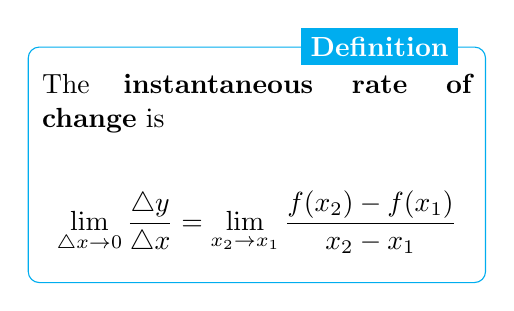
\begin{tikzpicture}
\node [rounded-box] (box){\begin{minipage}{0.45\textwidth}
    The \textbf{instantaneous rate of change} is

    $$\lim_{\triangle x \rightarrow 0} \frac{\triangle y}{\triangle x} = \lim_{x_2 \rightarrow x_1} \frac{f(x_2) - f(x_1)}{x_2 - x_1}$$
\end{minipage}};
\node[rounded-box-title, left=10pt] at (box.north east) {Definition};
\end{tikzpicture}

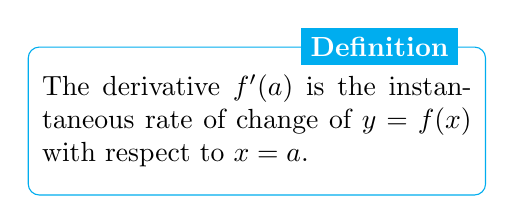
\begin{tikzpicture}
\node [rounded-box] (box){\begin{minipage}{0.45\textwidth}
    The derivative $f'(a)$ is the instantaneous rate of change of $y = f(x)$ with respect to $x = a$.
\end{minipage}};
\node[rounded-box-title, left=10pt] at (box.north east) {Definition};
\end{tikzpicture}

\switchcolumn

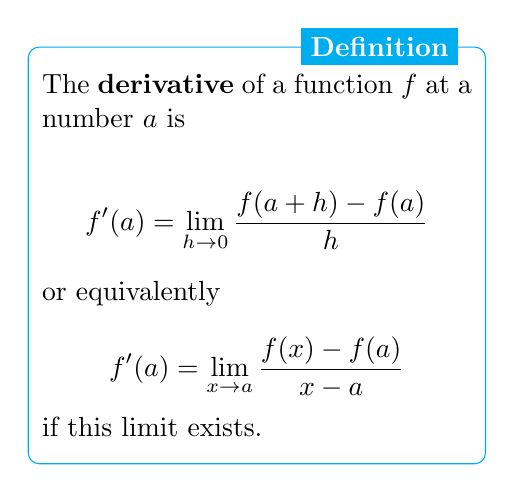
\begin{tikzpicture}
\node [rounded-box] (box){\begin{minipage}{0.45\textwidth}
    The \textbf{derivative} of a function $f$ at a number $a$ is

    $$f'(a) = \lim_{h \rightarrow 0} \frac{f(a + h) - f(a)}{h}$$

    or equivalently

    $$f'(a) = \lim_{x \rightarrow a} \frac{f(x) - f(a)}{x - a}$$

    if this limit exists.
\end{minipage}};
\node[rounded-box-title, left=10pt] at (box.north east) {Definition};
\end{tikzpicture}

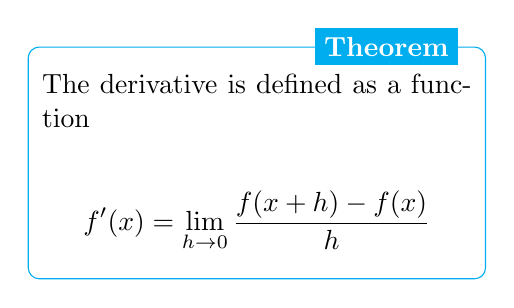
\begin{tikzpicture}
\node [rounded-box] (box){\begin{minipage}{0.45\textwidth}
    The derivative is defined as a function

    $$f'(x) = \lim_{h \rightarrow 0} \frac{f(x + h) - f(x)}{h}$$
\end{minipage}};
\node[rounded-box-title, left=10pt] at (box.north east) {Theorem};
\end{tikzpicture}

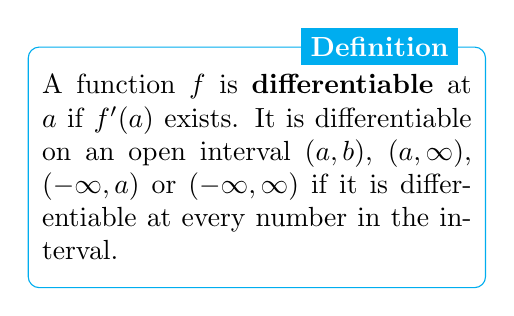
\begin{tikzpicture}
\node [rounded-box] (box){\begin{minipage}{0.45\textwidth}
    A function $f$ is \textbf{differentiable} at $a$ if $f'(a)$ exists. It is differentiable on an open interval $(a, b)$, $(a, \infty)$, $(-\infty, a)$ or $(-\infty, \infty)$ if it is differentiable at every number in the interval.
\end{minipage}};
\node[rounded-box-title, left=10pt] at (box.north east) {Definition};
\end{tikzpicture}

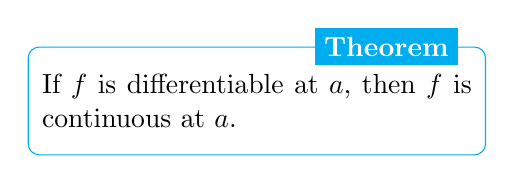
\begin{tikzpicture}
\node [rounded-box] (box){\begin{minipage}{0.45\textwidth}
    If $f$ is differentiable at $a$, then $f$ is continuous at $a$.
\end{minipage}};
\node[rounded-box-title, left=10pt] at (box.north east) {Theorem};
\end{tikzpicture}

\end{paracol}

\subsection{Linear Approximations and Differentials}

\begin{paracol}{2}

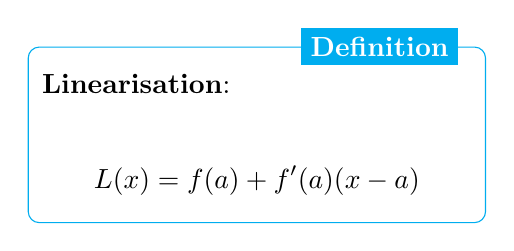
\begin{tikzpicture}
\node [rounded-box] (box){\begin{minipage}{0.45\textwidth}
    \textbf{Linearisation}:

    $$L(x) = f(a) + f'(a) (x - a)$$
\end{minipage}};
\node[rounded-box-title, left=10pt] at (box.north east) {Definition};
\end{tikzpicture}

\switchcolumn

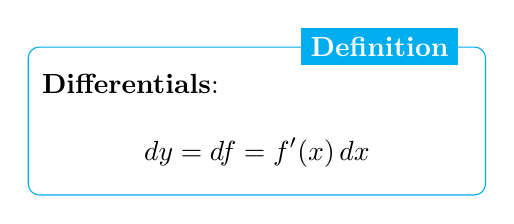
\begin{tikzpicture}
\node [rounded-box] (box){\begin{minipage}{0.45\textwidth}
    \textbf{Differentials}:

    $$dy = df = f'(x) \, dx$$
\end{minipage}};
\node[rounded-box-title, left=10pt] at (box.north east) {Definition};
\end{tikzpicture}

\end{paracol}

\newpage

\subsection{Extreme Values}

\begin{paracol}{2}

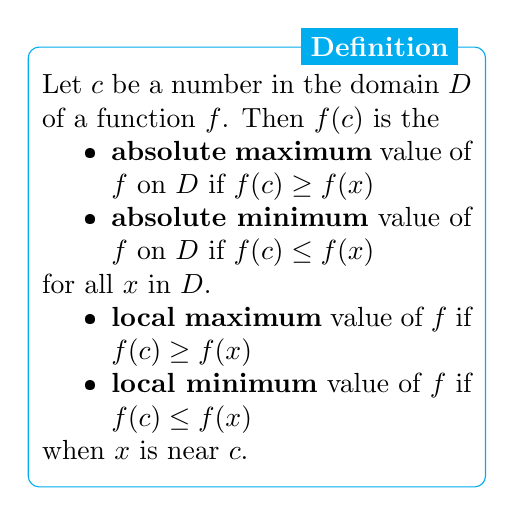
\begin{tikzpicture}
\node [rounded-box] (box){\begin{minipage}{0.45\textwidth}
    Let $c$ be a number in the domain $D$ of a function $f$. Then $f(c)$ is the

    \begin{itemize}
        \item \textbf{absolute maximum} value of $f$ on $D$ if $f(c) \geq f(x)$
        \item \textbf{absolute minimum} value of $f$ on $D$ if $f(c) \leq f(x)$
    \end{itemize}
    
    for all $x$ in $D$.

    \begin{itemize}
        \item \textbf{local maximum} value of $f$ if $f(c) \geq f(x)$
        \item \textbf{local minimum} value of $f$ if $f(c) \leq f(x)$
    \end{itemize}

     when $x$ is near $c$.
\end{minipage}};
\node[rounded-box-title, left=10pt] at (box.north east) {Definition};
\end{tikzpicture}

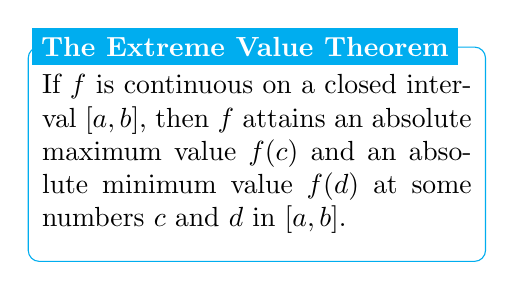
\begin{tikzpicture}
\node [rounded-box] (box){\begin{minipage}{0.45\textwidth}
    If $f$ is continuous on a closed interval $[a, b]$, then $f$ attains an absolute maximum value $f(c)$ and an absolute minimum value $f(d)$ at some numbers $c$ and $d$ in $[a, b]$.
\end{minipage}};
\node[rounded-box-title, left=10pt] at (box.north east) {The Extreme Value Theorem};
\end{tikzpicture}

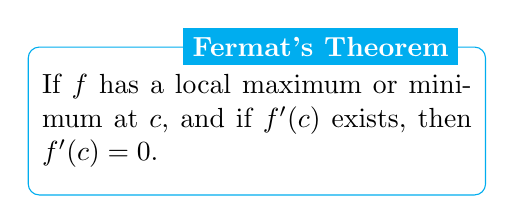
\begin{tikzpicture}
\node [rounded-box] (box){\begin{minipage}{0.45\textwidth}
    If $f$ has a local maximum or minimum at $c$, and if $f'(c)$ exists, then $f'(c) = 0$.
\end{minipage}};
\node[rounded-box-title, left=10pt] at (box.north east) {Fermat's Theorem};
\end{tikzpicture}

\switchcolumn

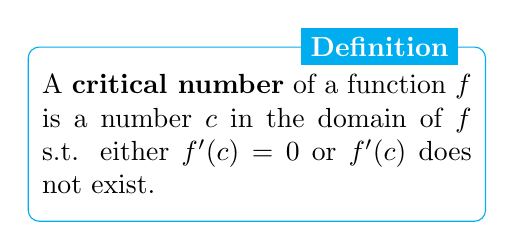
\begin{tikzpicture}
\node [rounded-box] (box){\begin{minipage}{0.45\textwidth}
    A \textbf{critical number} of a function $f$ is a number $c$ in the domain of $f$ s.t. either $f'(c) = 0$ or $f'(c)$ does not exist.
\end{minipage}};
\node[rounded-box-title, left=10pt] at (box.north east) {Definition};
\end{tikzpicture}

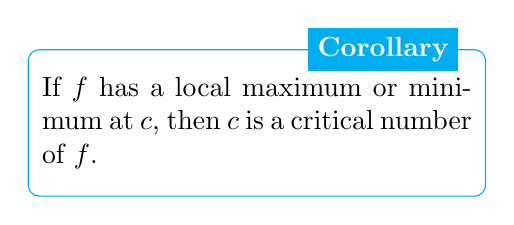
\begin{tikzpicture}
\node [rounded-box] (box){\begin{minipage}{0.45\textwidth}
    If $f$ has a local maximum or minimum at $c$, then $c$ is a critical number of $f$.
\end{minipage}};
\node[rounded-box-title, left=10pt] at (box.north east) {Corollary};
\end{tikzpicture}

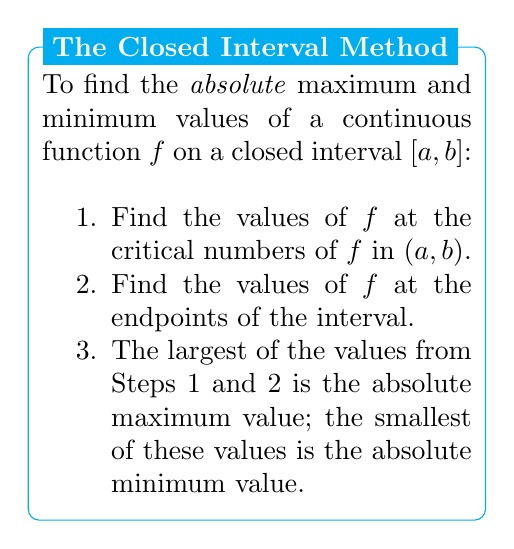
\begin{tikzpicture}
\node [rounded-box] (box){\begin{minipage}{0.45\textwidth}
    To find the \textit{absolute} maximum and minimum values of a continuous function $f$ on a closed interval $[a, b]$: \\

    \begin{enumerate}
        \item Find the values of $f$ at the critical numbers of $f$ in $(a, b)$.
        \item Find the values of $f$ at the endpoints of the interval.
        \item The largest of the values from Steps 1 and 2 is the absolute maximum value; the smallest of these values is the absolute minimum value.
    \end{enumerate}
\end{minipage}};
\node[rounded-box-title, left=10pt] at (box.north east) {The Closed Interval Method};
\end{tikzpicture}

\end{paracol}

\subsection{The Mean Value Theorem}

\begin{paracol}{2}

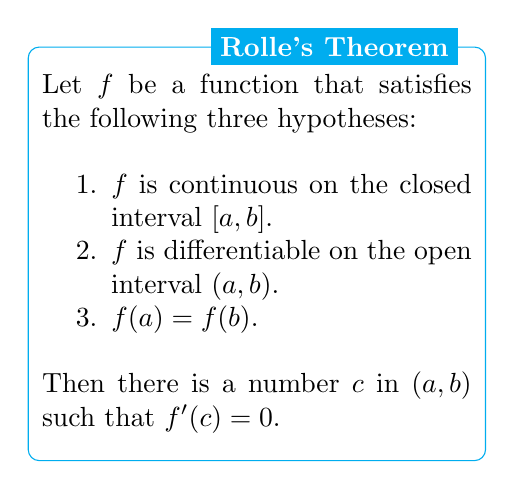
\begin{tikzpicture}
\node [rounded-box] (box){\begin{minipage}{0.45\textwidth}
    Let $f$ be a function that satisfies the following three hypotheses: \\

    \begin{enumerate}
        \item $f$ is continuous on the closed interval $[a, b]$.
        \item $f$ is differentiable on the open interval $(a, b)$.
        \item $f(a) = f(b)$. \\
    \end{enumerate}

    Then there is a number $c$ in $(a, b)$ such that $f'(c) = 0$.
\end{minipage}};
\node[rounded-box-title, left=10pt] at (box.north east) {Rolle's Theorem};
\end{tikzpicture}

\begin{tikzpicture}
\node [rounded-box] (box){\begin{minipage}{0.45\textwidth}
    If $f'(x) = 0$ for all $x$ in an interval $(a, b)$, then $f$ is constant on $(a, b)$.
\end{minipage}};
\node[rounded-box-title, left=10pt] at (box.north east) {Theorem};
\end{tikzpicture}

\begin{tikzpicture}
\node [rounded-box] (box){\begin{minipage}{0.45\textwidth}
    If $f'(x) = g'(x)$ for all $x$ in an interval $(a, b)$, then $f - g$ is constant on $(a, b)$; that is, $f(x) = g(x) + c$ where $c$ is a constant.
\end{minipage}};
\node[rounded-box-title, left=10pt] at (box.north east) {Corollary};
\end{tikzpicture}

\switchcolumn

\begin{tikzpicture}
\node [rounded-box] (box){\begin{minipage}{0.45\textwidth}
    Let $f$ be a function that satisfies the following hypotheses:

    \begin{enumerate}
        \item $f$ is continuous on the closed interval $[a, ]$.
        \item $f$ is differentiable on the open interval $(a, b)$.
    \end{enumerate}

    Then there is a number $c$ in $(a, b)$ such that

    $$f'(c) = \frac{f(b) - f(a)}{b - a}$$

    or, equivalently,

    $$f(b) - f(a) = f'(c)(b - a)$$
\end{minipage}};
\node[rounded-box-title, left=10pt] at (box.north east) {The Mean Value Theorem};
\end{tikzpicture}

\begin{tikzpicture}
\node [rounded-box] (box){\begin{minipage}{0.45\textwidth}
    Suppose that the functions $f$ and $g$ are continuous on $[a, b]$ and differentiable on $(a, b)$, and $g'(x) \neq 0$ for all $x$ in $(a, b)$. Then there is a number $c$ in $(a, b)$ such that

    $$\frac{f'(c)}{g'(c)} = \frac{f(b) - f(a)}{g(b) - g(a)}$$
\end{minipage}};
\node[rounded-box-title, left=10pt] at (box.north east) {Cauchy's Mean Value Theorem};
\end{tikzpicture}

\end{paracol}

Note: Given the special case in which $g(x) = x$, then $g'(c) = 1$ and Cauchy's Mean Value Theorem is the Mean Value Theorem.

\subsection{Derivatives and the Shapes of Graphs}

\begin{paracol}{2}

\begin{tikzpicture}
\node [rounded-box] (box){\begin{minipage}{0.45\textwidth}
    \begin{itemize}
        \item If $f'(x) > 0$, then $f$ is increasing on that interval.
        \item If $f'(x) < 0$, then $f$ is decreasing on that interval.
    \end{itemize}
\end{minipage}};
\node[rounded-box-title, left=10pt] at (box.north east) {Increasing / Decreasing Test};
\end{tikzpicture}

\begin{tikzpicture}
\node [rounded-box] (box){\begin{minipage}{0.45\textwidth}
    Suppose $c$ is a critical number of a continuous function $f$.

    \begin{itemize}
        \item Local max: $f'$ changes from positive to negative.
        \item Local min: $f'$ changes from negative to positive.
        \item Neither: $f'$ does not change sign at $c$.
    \end{itemize}
\end{minipage}};
\node[rounded-box-title, left=10pt] at (box.north east) {The First Derivative Test};
\end{tikzpicture}

\begin{tikzpicture}
\node [rounded-box] (box){\begin{minipage}{0.45\textwidth}
    If the graph of $f$ lies above / below all of its tangents on an interval $I$, it is \textbf{concave upward / downward} on $I$.
\end{minipage}};
\node[rounded-box-title, left=10pt] at (box.north east) {Definition};
\end{tikzpicture}

\switchcolumn

\begin{tikzpicture}
\node [rounded-box] (box){\begin{minipage}{0.45\textwidth}
    \begin{itemize}
        \item Concave upward on $I$: $f''(x) > 0$ for all $x$ in $I$.
        \item Concave downward on $I$: $f''(x) < 0$ for all $x$ in $I$.
    \end{itemize}
\end{minipage}};
\node[rounded-box-title, left=10pt] at (box.north east) {Concavity Test};
\end{tikzpicture}

\begin{tikzpicture}
\node [rounded-box] (box){\begin{minipage}{0.45\textwidth}
    A point $P$ on a curve $y = f(x)$ is called an \textbf{inflection point} if $f$ is continuous there and the curve changes from concave upward to concave downward or from concave downward to concave upward at $P$.
\end{minipage}};
\node[rounded-box-title, left=10pt] at (box.north east) {Definition};
\end{tikzpicture}

\begin{tikzpicture}
\node [rounded-box] (box){\begin{minipage}{0.45\textwidth}
    \begin{itemize}
        \item Local minimum at $c$: $f'(c) = 0$ and $f''(c) > 0$.
        \item Local maximum at $c$: $f'(c) = 0$ and $f''(c) < 0$.
    \end{itemize}
\end{minipage}};
\node[rounded-box-title, left=10pt] at (box.north east) {The Second Derivative Test};
\end{tikzpicture}

\end{paracol}
 \newpage
\section{Integration}

\subsection{Areas and Distances}

\begin{tikzpicture}
\node [rounded-box] (box){\begin{minipage}{0.975\textwidth}
    The area $A$ of the region $S$ that lies under the graph of the continuous function $f$ is the limit of the sum of the areas of approximating rectangles:

    $$A = \lim_{n \rightarrow \infty} R_n = \lim_{n \rightarrow \infty} [f(x_1) \triangle x + f(x_2) \triangle x + \dots + f(x_n) \triangle x]$$
\end{minipage}};
\node[rounded-box-title, left=10pt] at (box.north east) {Definition};
\end{tikzpicture}

\subsection{The Definite Integral}

\begin{paracol}{2}

\begin{tikzpicture}
\node [rounded-box] (box){\begin{minipage}{0.45\textwidth}
    If $f$ is a function defined on $[a, b]$, the \textbf{definite integral} of $f$ from $a$ to $b$ is the number

    $$\int_a^b f(x) \, dx = \lim_{\max{\triangle x_i} \rightarrow 0} \sum_{i=1}^n f(x_i^*) \triangle x_i$$

    provided that this limit exists.
\end{minipage}};
\node[rounded-box-title, left=10pt] at (box.north east) {Definition};
\end{tikzpicture}

\switchcolumn

\begin{tikzpicture}
\node [rounded-box] (box){\begin{minipage}{0.45\textwidth}
    \vspace{5pt}

    If $f$ is continuous on $[a, b]$, or if $f$ has only a finite number of jump discontinuities, then $f$ is \textbf{integrable} on $[a, b]$; that is, the definite integral $\int_a^b f(x) \, dx$ exists.

    \vspace{5pt}
\end{minipage}};
\node[rounded-box-title, left=10pt] at (box.north east) {Theorem};
\end{tikzpicture}

\switchcolumn

\begin{tikzpicture}
\node [rounded-box] (box){\begin{minipage}{0.45\textwidth}
    If $f$ is integrable on $[a, b]$, then

    $$\int_a^b f(x) \, dx = \lim_{n \rightarrow \infty} \sum_{i=1}^n f(x_i) \triangle x$$

    where $\triangle x = \frac{b - a}{n}$ and $x_i = a + i \triangle x$.
\end{minipage}};
\node[rounded-box-title, left=10pt] at (box.north east) {Theorem};
\end{tikzpicture}

\switchcolumn

\begin{tikzpicture}
\node [rounded-box] (box){\begin{minipage}{0.45\textwidth}
    $$\int_a^b f(x) \, dx \approx \sum_{i=1}^n f(\bar{x}_i) \triangle x = \triangle x [f(\bar{x}_1) + \dots + f(\bar{x}_n)]$$

    where $\triangle x = \frac{b - a}{n}$ \\

    and $\bar{x}_i = \frac{1}{2} (x_{i-1} + x_i)$ is the midpoint of $[x_{i-1}, x_i]$. \\
\end{minipage}};
\node[rounded-box-title, left=10pt] at (box.north east) {Midpoint Rule};
\end{tikzpicture}

\switchcolumn

\begin{tikzpicture}
\node [rounded-box] (box){\begin{minipage}{0.45\textwidth}
    \textbf{Properties of the integral}: \\

    \begin{enumerate}
        \item $\int_a^b c \, dx = c(b - a)$, where $c$ is any constant \\

        \item $\int_a^b [f(x) + g(x)] \, dx = \int_a^b f(x) \, dx + \int_a^b g(x) \, dx$ \\

        \item $\int_a^b c f(x) \, dx = c \int_a^b f(x) \, dx$, where $c$ is any constant \\

        \item $\int_a^b [f(x) - g(x)] \, dx = \int_a^b f(x) \, dx - \int_a^b g(x) \, dx$ \\

        \item $\int_a^c f(x) \, dx + \int_c^b f(x) \, dx = \int_a^b f(x) \, dx$
    \end{enumerate}
\end{minipage}};
\node[rounded-box-title, left=10pt] at (box.north east) {Definition};
\end{tikzpicture}

\switchcolumn

\begin{tikzpicture}
\node [rounded-box] (box){\begin{minipage}{0.45\textwidth}
    \textbf{Comparison properties of the integral}: \\

    \begin{enumerate}
        \item If $f(x) \geq 0$ for $a \leq x \leq b$, then $\int_a^b f(x) \, dx \geq 0$. \\

        \item If $f(x) \geq g(x)$ for $a \leq x \leq b$, then $\int_a^b f(x) \, dx \geq \int_a^b g(x) \, dx$. \\

        \item If $m \leq f(x) \leq M$ for $a \leq x \leq b$, then

        $$m(b - a) \leq \int_a^b f(x) \, dx \leq M(b - a)$$
    \end{enumerate}
\end{minipage}};
\node[rounded-box-title, left=10pt] at (box.north east) {Definition};
\end{tikzpicture}

\switchcolumn

\begin{tikzpicture}
\node [rounded-box] (box){\begin{minipage}{0.45\textwidth}
    If $f$ is continuous on the interval $[a, b]$, then

    $$\int_a^b f(x) \, dx = F(b) - F(a)$$

    where $F$ is any \textbf{antiderivative} of $f$, that is, $F'(x) = f(x)$ for all $x$ in an interval $I$.
\end{minipage}};
\node[rounded-box-title, left=10pt] at (box.north east) {Evaluation Theorem};
\end{tikzpicture}

\switchcolumn

\begin{tikzpicture}
\node [rounded-box] (box){\begin{minipage}{0.45\textwidth}
    The integral of a rate of change is the net change:

    $$\int_a^b F'(x) \, dx = F(b) - F(a)$$
\end{minipage}};
\node[rounded-box-title, left=10pt] at (box.north east) {Net Change Theorem};
\end{tikzpicture}

\end{paracol}

\subsection{The Fundamental Theorem of Calculus}

\begin{paracol}{2}

\begin{tikzpicture}
\node [rounded-box] (box){\begin{minipage}{0.45\textwidth}
    Suppose $f$ is continuous on $[a, b]$. \\

    \begin{enumerate}
        \item If $g(x) = \int_a^x f(t) \, dt$, then $g'(x) = f(x)$. \\

        \item $\int_a^b f(x) \, dx = F(b) - F(a)$, where $F$ is any antiderivative of $f$; that is, $F' = f$.
    \end{enumerate}
\end{minipage}};
\node[rounded-box-title, left=10pt] at (box.north east) {The Fundamental Theorem of Calculus};
\end{tikzpicture}

\switchcolumn

\begin{tikzpicture}
\node [rounded-box] (box){\begin{minipage}{0.45\textwidth}
    If $f$ is continuous on $[a, b]$, then there exists a number $c$ in $[a, b]$ such that $f(c)$ is the \textbf{average value} of a function:

    $$f(c) = f_\text{ave} = \frac{1}{b - a} \int_a^b f(x) \, dx$$

    $$\text{that is, } \qquad \qquad \int_a^b f(x) \, dx = f(c) (b - a) \qquad \qquad \qquad$$
\end{minipage}};
\node[rounded-box-title, left=10pt] at (box.north east) {The Mean Value Theorem for Integrals};
\end{tikzpicture}

\end{paracol}

\subsection{Improper Integrals}

\begin{paracol}{2}

\begin{tikzpicture}
\node [rounded-box] (box){\begin{minipage}{0.45\textwidth}
    \textbf{Improper integrals of type 1}:

    \begin{itemize}
        \item If $\int_a^t f(x) \, dx$ exists for every number $t \geq a$, then

        $$\int_a^\infty f(x) \, dx = \lim_{t \rightarrow \infty} \int_a^t f(x) \, dx$$

        provided this limit exists (as a finite number).

        \item If $\int_t^b f(x) \, dx$ exists for every number $t \leq b$, then

        $$\int_{-\infty}^b f(x) \, dx = \lim_{t \rightarrow -\infty} \int_t^b f(x) \, dx$$

        provided this limit exists (as a finite number).
    \end{itemize}
\end{minipage}};
\node[rounded-box-title, left=10pt] at (box.north east) {Definition};
\end{tikzpicture}

\begin{tikzpicture}
\node [rounded-box] (box){\begin{minipage}{0.45\textwidth}
    The improper integrals $\int_a^\infty f(x) \, dx$ and $\int_{-\infty}^b f(x) \, dx$ are called \textbf{convergent} if the corresponding limit exists and \textbf{divergent} if the limit does not exist.
\end{minipage}};
\node[rounded-box-title, left=10pt] at (box.north east) {Theorem};
\end{tikzpicture}

\begin{tikzpicture}
\node [rounded-box] (box){\begin{minipage}{0.45\textwidth}
    If $\int_a^\infty f(x) \, dx$ and $\int_{-\infty}^a f(x) \, dx$ are called convergent, then

    $$\int_{-\infty}^\infty f(x) \, dx = \int_{-\infty}^a f(x) \, dx + \int_a^\infty f(x) \, dx$$
\end{minipage}};
\node[rounded-box-title, left=10pt] at (box.north east) {Theorem};
\end{tikzpicture}

\switchcolumn

\begin{tikzpicture}
\node [rounded-box] (box){\begin{minipage}{0.45\textwidth}
    \textbf{Improper integrals of type 2}:

    \begin{itemize}
        \item If $f$ is continuous on $[a, b)$ and discontinuous at $b$,

        $$\int_a^b f(x) \, dx = \lim_{t \rightarrow b^-} \int_a^t f(x) \, dx$$

        if this limit exists (as a finite number).

        \item If $f$ is continuous on $(a, b]$ and discontinuous at $a$,

        $$\int_a^b f(x) \, dx = \lim_{t \rightarrow a^+} \int_t^b f(x) \, dx$$

        if this limit exists (as a finite number).
    \end{itemize}
\end{minipage}};
\node[rounded-box-title, left=10pt] at (box.north east) {Definition};
\end{tikzpicture}

\begin{tikzpicture}
\node [rounded-box] (box){\begin{minipage}{0.45\textwidth}
    The improper integrals $\int_a^b f(x) \, dx$ is called \textbf{convergent} if the corresponding limit exists and \textbf{divergent} if the limit does not exist.
\end{minipage}};
\node[rounded-box-title, left=10pt] at (box.north east) {Theorem};
\end{tikzpicture}

\begin{tikzpicture}
\node [rounded-box] (box){\begin{minipage}{0.45\textwidth}
    If $f$ has a discontinuity at $c$, where $a < c < b$, and both $\int_a^c f(x) \, dx$ and $\int_c^b f(x) \, dx$ are convergent, then we define

    $$\int_a^b f(x) \, dx = \int_a^c f(x) \, dx + \int_c^b f(x) \, dx$$
\end{minipage}};
\node[rounded-box-title, left=10pt] at (box.north east) {Theorem};
\end{tikzpicture}

\end{paracol}

\begin{tikzpicture}
\node [rounded-box] (box){\begin{minipage}{0.975\textwidth}
\begin{center}
    $\int_1^\infty \frac{1}{x^p} \, dx$ is convergent if $p > 1$ and divergent if $p \leq 1$.
\end{center}
\end{minipage}};
\node[rounded-box-title, left=10pt] at (box.north east) {Theorem};
\end{tikzpicture}

\textbf{Proof}: Suppose $T_n(x)$ is the $n^\text{th}$ Taylor polynomial of a function $f(x)$. Then $\int T_n(x) \, dx$ is the $(n + 1)^\text{st}$ Taylor polynomial of an anti-derivative $F(x)$ of $f(x)$. For $a > 0$:

$$
\int_a^\infty \frac{1}{x^p} \, dx \quad \begin{cases}
    \text{diverges} & \text{if } p \leq 1 \\
    \text{converges to } \frac{a^{-p + 1}}{p - 1} & \text{if } p > 1
\end{cases}
\qquad \qquad
\int_0^a \frac{1}{x^p} \, dx \quad \begin{cases}
    \text{diverges} & \text{if } p \geq 1 \\
    \text{converges to } \frac{a^{1 - p}}{1 - p} & \text{if } p < 1
\end{cases}
$$

\begin{tikzpicture}
\node [rounded-box] (box){\begin{minipage}{0.975\textwidth}
    Suppose that $f$ and $g$ are continuous functions with $f(x) \geq g(x) \geq 0$ for $x \geq a$. \\

    \begin{itemize}
        \item If $\int_a^\infty f(x) \, dx$ is convergent, then $\int_a^\infty g(x) \, dx$ is convergent. \\

        \item If $\int_a^\infty g(x) \, dx$ is divergent, then $\int_a^\infty f(x) \, dx$ is divergent.
    \end{itemize}
\end{minipage}};
\node[rounded-box-title, left=10pt] at (box.north east) {Comparison Theorem};
\end{tikzpicture}

\subsection{Techniques of Integration}

\begin{paracol}{2}

\begin{tikzpicture}
\node [rounded-box] (box){\begin{minipage}{0.45\textwidth}
    If $g'$ is continuous on $[a, b]$ and $f$ is continuous on the range of $u = g(x)$, then

    $$\int_a^b f(g(x)) g'(x) \, dx = \int_{g(a)}^{g(b)} f(u) \, du$$
\end{minipage}};
\node[rounded-box-title, left=10pt] at (box.north east) {Substitution Rule for Definite Integrals};
\end{tikzpicture}

\switchcolumn

\begin{tikzpicture}
\node [rounded-box] (box){\begin{minipage}{0.45\textwidth}
    Suppose $f$ is continuous on $[-a, a]$. \\

    \begin{itemize}
        \item If $f$ is even, $f(-x) = f(x)$, then $\int_{-a}^a f(x) \, dx = 2 \int_0^a f(x) \, dx$.

        \item If $f$ is odd, $f(-x) = -f(x)$, then $\int_{-a}^a f(x) \, dx = 0$.
    \end{itemize}
\end{minipage}};
\node[rounded-box-title, left=10pt] at (box.north east) {Integrals of Symmetric Functions};
\end{tikzpicture}

\end{paracol}

\begin{tikzpicture}
\node [rounded-box] (box){\begin{minipage}{0.975\textwidth}
    $$\qquad \qquad \int u \, dv = uv - \int v \, du \qquad \text{or, equivalently,} \qquad \int_a^b f(x) g'(x) \, dx = f(x) g(x) \Big|_a^b - \int_a^b g(x) f'(x) \, dx$$
\end{minipage}};
\node[rounded-box-title, left=10pt] at (box.north east) {Integration by Parts};
\end{tikzpicture}

\quad

\begin{center}
\begin{tabular}{c|c|c}
    Expression & Trigonometric Substitution & Identity \\[0.25cm]
    \hline
    & & \\[0.25cm]

    $\sqrt{a^2 - x^2}$ & $x = a \sin{\theta}, -\frac{\pi}{2} \leq \theta \leq \frac{\pi}{2}$ & $1 - \sin^2{\theta} = \cos^2{\theta}$ \\[0.5cm]

    $\sqrt{a^2 + x^2}$ & $x = a \tan{\theta}, -\frac{\pi}{2} < \theta < \frac{\pi}{2}$ & $1 + \tan^2{\theta} = \sec^2{\theta}$ \\[0.5cm]

    $\sqrt{x^2 - a^2}$ & $x = a \sec{\theta}, 0 \leq \theta \leq \frac{\pi}{2}$ or $\pi \leq \theta < \frac{3 \pi}{2}$ & $\sec^2{\theta} - 1 = \tan^2{\theta}$
\end{tabular}
\end{center}

\subsection{Applications of Integration}

\begin{paracol}{2}

\begin{tikzpicture}
\node [rounded-box] (box){\begin{minipage}{0.45\textwidth}
    The \textbf{area} $A$ of the region bounded by the curves $y = f(x), y = g(x)$ and the lines $x = a, x = b$, where $f$ and $g$ are continuous and $f(x) \geq g(x)$ for all $x$ in $[a, b]$, is

    $$A = \int_a^b [f(x) - g(x)] \, dx$$
\end{minipage}};
\node[rounded-box-title, left=10pt] at (box.north east) {Definition};
\end{tikzpicture}

\switchcolumn

\begin{tikzpicture}
\node [rounded-box] (box){\begin{minipage}{0.45\textwidth}
    Let $S$ be a solid that lies between $x = a$ and $x = b$. If the cross-sectional area of $S$ in the plane $P_x$, through $x$ and perpendicular to the $x$-axis, is $A(x)$, where $A$ is an integrable function, then the \textbf{volume} of $S$ is

    $$V = \lim_{\max{\triangle x_i} \rightarrow 0} \sum_{i=1}^n A(x_i^*) \triangle x_i = \int_a^b A(x) \, dx$$
\end{minipage}};
\node[rounded-box-title, left=10pt] at (box.north east) {Definition};
\end{tikzpicture}

\switchcolumn

\begin{tikzpicture}
\node [rounded-box] (box){\begin{minipage}{0.45\textwidth}
    \textbf{Surface area}: Where $f$ is positive and has a continuous derivative, the area of the surface obtained by rotating the curve $y = f(x), a \leq x \leq b,$ about the $x$-axis as

    \vspace{-10pt}

    $$S = \int_a^b 2 \pi \, f(x) \, \sqrt{1 + [f'(x)]^2} \, dx = \int_a^b 2 \pi \, y \, \sqrt{1 + \Big( \frac{dy}{dx} \Big)^2} \, dx$$

    If the curve is described as $x = g(y), c \leq y \leq d,$ then the formula for the surface area becomes

    \vspace{-10pt}

    $$S = \int_c^d 2 \pi \, g(y) \, \sqrt{1 + [g'(y)]^2} \, dy = \int_c^d 2 \pi \, x \, \sqrt{1 + \Big( \frac{dx}{dy} \Big)^2} \, dy$$
\end{minipage}};
\node[rounded-box-title, left=10pt] at (box.north east) {Definition};
\end{tikzpicture}

\switchcolumn

\begin{tikzpicture}
\node [rounded-box] (box){\begin{minipage}{0.45\textwidth}
    \textbf{Arc length}: If $f'$ is continuous on $[a, b]$, then the length of the curve $y = f(x), a \leq x \leq b$, is

    \vspace{-5pt}

    $$L = \int_a^b \sqrt{1 + [f'(x)]^2} \, dx = \int_a^b \sqrt{1 + \Big( \frac{dy}{dx} \Big)^2} \, dx$$

    If $g'$ is continuous on $[c, d]$, then the length of the curve $x = g(y), c \leq x \leq d$, is

    \vspace{-10pt}

    $$L = \int_c^d \sqrt{1 + [g'(y)]^2} \, dy = \int_c^d \sqrt{1 + \Big( \frac{dx}{dy} \Big)^2} \, dy$$
\end{minipage}};
\node[rounded-box-title, left=10pt] at (box.north east) {Definition};
\end{tikzpicture}

\switchcolumn

\begin{tikzpicture}
\node [rounded-box] (box){\begin{minipage}{0.45\textwidth}
    If a curve $C$ is described by the \textbf{parametric equations} $x = f(t), y = g(t)$ and is traversed once as $t$ increases from $\alpha$ to $\beta$, then the area under the curve is

    $$A = \int_a^b y \, dx = \int_\alpha^\beta g(t) f'(t) \, dt$$
\end{minipage}};
\node[rounded-box-title, left=10pt] at (box.north east) {Definition};
\end{tikzpicture}

\switchcolumn

\begin{tikzpicture}
\node [rounded-box] (box){\begin{minipage}{0.45\textwidth}
    If a curve $C$ is described by the \textbf{parametric equations} $x = f(t), y = g(t), \alpha \leq t \leq \beta$, where $f'$ and $g'$ are continuous on $[ \alpha, \beta]$ and $C$ is transversed exactly once as $t$ increases from $\alpha$ to $\beta$, then the length of $C$ is

    $$L = \int_\alpha^\beta \sqrt{\Big(\frac{dx}{dt}\Big)^2 + \Big(\frac{dy}{dt}\Big)^2} \, dt$$
\end{minipage}};
\node[rounded-box-title, left=10pt] at (box.north east) {Definition};
\end{tikzpicture}

\switchcolumn

\begin{tikzpicture}
\node [rounded-box] (box){\begin{minipage}{0.45\textwidth}
    In \textbf{polar coordinates},

    $$A = \int_a^b \frac{1}{2} [f(\theta)]^2 \, d\theta = \int_a^b \frac{1}{2} r^2 \, d\theta$$
\end{minipage}};
\node[rounded-box-title, left=10pt] at (box.north east) {Definition};
\end{tikzpicture}

\switchcolumn

\begin{tikzpicture}
\node [rounded-box] (box){\begin{minipage}{0.45\textwidth}
    In \textbf{polar coordinates},

    $$L = \int_a^b \sqrt{r^2 + \Big( \frac{dr}{d\theta} \Big)^2} \, d\theta$$
\end{minipage}};
\node[rounded-box-title, left=10pt] at (box.north east) {Definition};
\end{tikzpicture}

\end{paracol}

\section{Transcendental Functions}

Transcendental functions are non-algebraic functions that cannot be expressed as a finite combination of algebraic operations such as addition, subtraction, multiplication, division, raising to a power, and extracting roots. In other words, they are functions that are not solutions to polynomial equations.

\subsection{The Natural Logarithm}

\begin{tikzpicture}
\node [rounded-box] (box){\begin{minipage}{0.975\textwidth}
    The natural logarithmic function is the function defined by

    $$\ln{x} = \int_1^x \frac{1}{t} \, dt, \quad x > 0$$
\end{minipage}};
\node[rounded-box-title, left=10pt] at (box.north east) {Definition};
\end{tikzpicture}

The existence of this function depends on the fact that the integral of a continuous function always exists.

\begin{itemize}
    \item For $x > 1$, then $\ln{x}$ can be interpreted geometrically as the area under the hyperbola $y = \frac{1}{t}$ from $t = 1$ to $t = x$.
    \item For $x = 1$, $\ln{1} = \int_1^1 \frac{1}{t} \, dt = 0$
    \item For $0 < x < 1$, $ln{x} = \int_1^x \frac{1}{t} \, dt = - \int_x^1 \frac{1}{t} \, dt < 0$ and so $\ln{x}$ is the negative of the area under the hyperbola on that interval.
\end{itemize}

\begin{paracol}{2}

\begin{tikzpicture}
\node [rounded-box] (box){\begin{minipage}{0.45\textwidth}
    \vspace{-5pt}

    $$\frac{d}{dx}(\ln{x}) = \frac{1}{x}$$

    \vspace{-5pt}
\end{minipage}};
\node[rounded-box-title, left=10pt] at (box.north east) {Corollary};
\end{tikzpicture}

\switchcolumn

\begin{tikzpicture}
\node [rounded-box] (box){\begin{minipage}{0.45\textwidth}
    $$\lim_{x \rightarrow \infty} \ln{x} = \infty \qquad \lim_{x \rightarrow 0^+} \ln{x} = -\infty$$
\end{minipage}};
\node[rounded-box-title, left=10pt] at (box.north east) {Definition};
\end{tikzpicture}

\switchcolumn

\begin{tikzpicture}
\node [rounded-box] (box){\begin{minipage}{0.45\textwidth}
    $e$ is the number such that $\ln{e} = 1$.

    $$e = \lim_{x \rightarrow 0} (1+x)^{1/x}$$
\end{minipage}};
\node[rounded-box-title, left=10pt] at (box.north east) {Definition};
\end{tikzpicture}

\switchcolumn

\begin{tikzpicture}
\node [rounded-box] (box){\begin{minipage}{0.45\textwidth}
    \textbf{Laws of Logarithms}:

    \vspace{-10pt}

    $$\ln{xy} = \ln{x} + \ln{y} \qquad \ln{\frac{x}{y}} = \ln{x} - \ln{y} \qquad \ln{x^r} = r \ln{x}$$
\end{minipage}};
\node[rounded-box-title, left=10pt] at (box.north east) {Definition};
\end{tikzpicture}

\end{paracol}

\subsection{The Natural Exponential Function}

\begin{paracol}{2}

Since $\ln$ is an increasing function, it is one-to-one and therefore has an inverse function.

\begin{tikzpicture}
\node [rounded-box] (box){\begin{minipage}{0.45\textwidth}
    $$e^x = y \quad \iff \quad \ln{y} = x$$
\end{minipage}};
\node[rounded-box-title, left=10pt] at (box.north east) {Definition};
\end{tikzpicture}

\begin{tikzpicture}
\node [rounded-box] (box){\begin{minipage}{0.45\textwidth}
    $$e^{\ln{x}} = x, \quad x > 0 \qquad \ln{e^x} = x \text{ for all } x$$
\end{minipage}};
\node[rounded-box-title, left=10pt] at (box.north east) {Definition};
\end{tikzpicture}

\switchcolumn

\begin{tikzpicture}
\node [rounded-box] (box){\begin{minipage}{0.45\textwidth}
    \textbf{Laws of Exponents}: \\

    If $x, y$ are real numbers and $r$ is rational, then

    $$e^{x + y} = e^x e^y \qquad e^{x - y} = \frac{e^x}{e^y} \qquad (e^x)^r = e^{rx}$$

    If $x, y$ are real numbers and $a, b > 0$, then

    $$a^{x + y} = a^x a^y \quad a^{x - y} = \frac{a^x}{a^y} \quad (a^x)^y = a^{xy} \quad (ab)^x = a^x b^x$$
\end{minipage}};
\node[rounded-box-title, left=10pt] at (box.north east) {Definition};
\end{tikzpicture}

\end{paracol}

\begin{tikzpicture}
\node [rounded-box] (box){\begin{minipage}{0.975\textwidth}
    \textbf{Properties of the natural exponential function}: The exponential function $f(x) = e^x$ is a continuous function with domain $\mathbb{R}$ and range $(0, \infty)$.

    Thus, $e^x > 0$ for all $x$, $\lim_{x \rightarrow -\infty} e^x = 0$, $\lim_{x \rightarrow \infty} e^x = \infty$.

    The $x$-axis is a horizontal asymptote of $f(x) = e^x$.
\end{minipage}};
\node[rounded-box-title, left=10pt] at (box.north east) {Definition};
\end{tikzpicture}

\subsection{General Logarithmic Functions}

\begin{tikzpicture}
\node [rounded-box] (box){\begin{minipage}{0.975\textwidth}
    If $a > 0$ and $a \neq 1$, then $f(x) = a^x$ is a one-to-one function. Its inverse function is called the logarithmic function with base $a$:

    $$\log_a{x} = y \quad \iff \quad a^y = x$$

    $$\frac{d}{dx}(\log_a{x}) = \frac{1}{x \ln{a}}$$
\end{minipage}};
\node[rounded-box-title, left=10pt] at (box.north east) {Definition};
\end{tikzpicture}

\begin{paracol}{2}

\begin{tikzpicture}
\node [rounded-box] (box){\begin{minipage}{0.45\textwidth}
    $$\log_a(a^x) = x \text{ for all } x \in \mathbb{R}$$
\end{minipage}};
\node[rounded-box-title, left=10pt] at (box.north east) {Definition};
\end{tikzpicture}

\switchcolumn

\begin{tikzpicture}
\node [rounded-box] (box){\begin{minipage}{0.45\textwidth}
    $$a^{\log_a{x}} = x \text{ for all } x > 0$$
\end{minipage}};
\node[rounded-box-title, left=10pt] at (box.north east) {Definition};
\end{tikzpicture}

\begin{tikzpicture}
\node [rounded-box] (box){\begin{minipage}{0.45\textwidth}
    $$\log_a(xy) = \log_a(x) + \log_a(y)$$
\end{minipage}};
\node[rounded-box-title, left=10pt] at (box.north east) {Definition};
\end{tikzpicture}

\switchcolumn

\begin{tikzpicture}
\node [rounded-box] (box){\begin{minipage}{0.45\textwidth}
    $$\log_a(x / y) = \log_a(x) - \log_a(y)$$
\end{minipage}};
\node[rounded-box-title, left=10pt] at (box.north east) {Definition};
\end{tikzpicture}

\switchcolumn

\begin{tikzpicture}
\node [rounded-box] (box){\begin{minipage}{0.45\textwidth}
    If $a > 1$, then

    $$\lim_{x \rightarrow \infty} \log_a{x} = \infty \qquad \text{and} \qquad \lim_{x \rightarrow 0^+} \log_a{x} = -\infty$$
\end{minipage}};
\node[rounded-box-title, left=10pt] at (box.north east) {Definition};
\end{tikzpicture}

\switchcolumn

\begin{tikzpicture}
\node [rounded-box] (box){\begin{minipage}{0.45\textwidth}
    For any positive number $a$ ($a \neq 1$),

    $$\log_a{x} = \frac{\ln{x}}{\ln{a}}$$
\end{minipage}};
\node[rounded-box-title, left=10pt] at (box.north east) {Change-of-Base Formula};
\end{tikzpicture}

\end{paracol}
 \newpage
\section{Sequences and Series}

\subsection{Sequences}

\begin{paracol}{2}

\begin{tikzpicture}
\node [rounded-box] (box){\begin{minipage}{0.45\textwidth}
    A sequence $\{a_n\}$ has the limit $L$ and we write

    $$\lim_{n \rightarrow \infty} = L \qquad \text{or} \qquad a_n \rightarrow L \text{ as } n \rightarrow \infty$$

    if we can make the terms $a_n$ as close to $L$ as we like by taking $n$ sufficiently large. \\

    If $\lim_{n \rightarrow \infty} a_n$ exists, we say the sequence \textbf{converges} (or is convergent). Otherwise, it \textbf{diverges} (or is divergent).
\end{minipage}};
\node[rounded-box-title, left=10pt] at (box.north east) {Definition};
\end{tikzpicture}

\begin{tikzpicture}
\node [rounded-box] (box){\begin{minipage}{0.45\textwidth}
    If $\lim_{x \rightarrow \infty} f(x) = L$ and $f(n) = a_n$ when $n$ is an integer, then $\lim_{n \rightarrow \infty} a_n = L$.
\end{minipage}};
\node[rounded-box-title, left=10pt] at (box.north east) {Theorem};
\end{tikzpicture}

\begin{tikzpicture}
\node [rounded-box] (box){\begin{minipage}{0.45\textwidth}
    \textbf{Limit Laws for Sequences}: If $\{a_n\}$ and $\{b_n\}$ are convergent sequences and $c$ is a constant, then

    $$\lim_{n \rightarrow \infty} (a_n + b_n) = \lim_{n \rightarrow \infty} a_n + \lim_{n \rightarrow \infty} b_n$$

    $$\lim_{n \rightarrow \infty} (a_n - b_n) = \lim_{n \rightarrow \infty} a_n - \lim_{n \rightarrow \infty} b_n$$

    $$\lim_{n \rightarrow \infty} c a_n = c \lim_{n \rightarrow \infty} a_n
    \qquad \qquad
    \lim_{n \rightarrow \infty} c = c$$

    $$\lim_{n \rightarrow \infty} (a_n b_n) = \lim_{n \rightarrow \infty} a_n \cdot \lim_{n \rightarrow \infty} a_n$$

    $$\lim_{n \rightarrow \infty} \frac{a_n}{b_n} = \frac{\lim_{n \rightarrow \infty} a_n}{\lim_{n \rightarrow \infty} b_n} \text{ if } \lim_{n \rightarrow \infty} b_n \neq 0$$

    $$\lim_{n \rightarrow \infty} a_n^p = [\lim_{n \rightarrow \infty} a_n]^p \text{ if } p > 0 \text{ and } a_n > 0$$
\end{minipage}};
\node[rounded-box-title, left=10pt] at (box.north east) {Theorem};
\end{tikzpicture}

\begin{tikzpicture}
\node [rounded-box] (box){\begin{minipage}{0.45\textwidth}
    If $a_n \leq b_n \leq c_n$ for $n \geq n_0$ and $\lim_{n \rightarrow \infty} a_n = \lim_{n \rightarrow \infty} c_n = L$, then $\lim_{n \rightarrow \infty} b_n = L$.
\end{minipage}};
\node[rounded-box-title, left=10pt] at (box.north east) {Theorem};
\end{tikzpicture}

\begin{tikzpicture}
\node [rounded-box] (box){\begin{minipage}{0.45\textwidth}
    If $\lim_{n \rightarrow \infty} | a_n | = 0$, then $\lim_{n \rightarrow \infty} a_n = 0$.
\end{minipage}};
\node[rounded-box-title, left=10pt] at (box.north east) {Theorem};
\end{tikzpicture}

\switchcolumn

\begin{tikzpicture}
\node [rounded-box] (box){\begin{minipage}{0.45\textwidth}
    If $\lim_{n \rightarrow \infty} a_n = L$ and the function $f$ is continuous at $L$, then

    $$\lim_{n \rightarrow \infty} f(a_n) = f(L)$$
\end{minipage}};
\node[rounded-box-title, left=10pt] at (box.north east) {Continuity and Convergence Theorem};
\end{tikzpicture}

\begin{tikzpicture}
\node [rounded-box] (box){\begin{minipage}{0.45\textwidth}
    The sequence $\{r^n\}$ is convergent if $-1 < r \leq 1$ and divergent for all other values of $r$.

    $$
    \lim_{n \rightarrow \infty} r^n = \begin{cases}
        0 & \text{if } -1 < r < 1 \\
        1 & \text{if } r = 1
    \end{cases}
    $$
\end{minipage}};
\node[rounded-box-title, left=10pt] at (box.north east) {Theorem};
\end{tikzpicture}

\begin{tikzpicture}
\node [rounded-box] (box){\begin{minipage}{0.45\textwidth}
    A sequence $\{a_n\}$ is called \textbf{increasing} if $a_n < a_{n+1}$ for all $n \geq 1$, that is, $a_1 < a_2 < a_3 < \dots$. It is called \textbf{decreasing} if $a_n > a_{n + 1}$ for all $n \geq 1$. \\

    A sequence is \textbf{monotonic} if it is either increasing or decreasing.
\end{minipage}};
\node[rounded-box-title, left=10pt] at (box.north east) {Definition};
\end{tikzpicture}

\begin{tikzpicture}
\node [rounded-box] (box){\begin{minipage}{0.45\textwidth}
    A sequence $\{a_n\}$ is \textbf{bounded above} if there is a number $M$ such that

    $$a_n \leq M \quad \text{for all } n \geq 1$$

    A sequence $\{a_n\}$ is \textbf{bounded below} if there is a number $m$ such that

    $$m \leq a_n \quad \text{for all } n \geq 1$$

    If a sequence is bounded above and below, then it is a \textbf{bounded sequence}.
\end{minipage}};
\node[rounded-box-title, left=10pt] at (box.north east) {Definition};
\end{tikzpicture}

\begin{tikzpicture}
\node [rounded-box] (box){\begin{minipage}{0.45\textwidth}
    Every bounded, monotonic sequence is convergent.
\end{minipage}};
\node[rounded-box-title, left=10pt] at (box.north east) {Monotonic Sequence Theorem};
\end{tikzpicture}

\end{paracol}

\subsection{Series}

\begin{paracol}{2}

\begin{tikzpicture}
\node [rounded-box] (box){\begin{minipage}{0.45\textwidth}
    Given a series $\sum_{n = 1}^\infty a_n = a_1 + a_2 + a_3 + \dots$, let $s_n$ denote its $n^\text{th}$ partial sum:

    $$s_n = \sum_{i = 1}^n a_i = a_1 + a_2 + \dots + a_n$$

    If the sequence $\{s_n\}$ is convergent and $\lim_{n \rightarrow \infty} s_n = s$ exists as a real number, then the series $\sum a_n$ is called \textbf{convergent}, and we write

    \vspace{-20pt}

    $$a_1 + a_2 + \dots + a_n + \dots = s \qquad \text{or} \qquad \sum_{n = 1}^\infty a_n = s$$

    The number $s$ is called the \textbf{sum} of the series. If the sequence $\{s_n\}$ is divergent, the series is called \textbf{divergent}.
\end{minipage}};
\node[rounded-box-title, left=10pt] at (box.north east) {Definition};
\end{tikzpicture}

\switchcolumn

\begin{tikzpicture}
\node [rounded-box] (box){\begin{minipage}{0.45\textwidth}
    The \textbf{geometric series} $\sum_{n = 1}^\infty a r^{n-1} = a + ar + ar^2 + \dots$ is divergent if $| r | \geq 1$; convergent if $| r | < 1$, and its sum is

    $$\sum_{n = 1}^\infty a r^{n-1} = \frac{a}{1 - r} \qquad | r | < 1$$
\end{minipage}};
\node[rounded-box-title, left=10pt] at (box.north east) {Definition};
\end{tikzpicture}

\textbf{Proof}: $s_n = 1 + a + a^2 + \dots + a^n, s_{n+1} = 1 + a + a^2 + \dots + a^n + a^{n+1}$. Then $s_n + a^{n+1} = 1 + a s_n \quad \Rightarrow \quad s_n (1 - a) = 1 - a^{n+1} \quad \Rightarrow \quad s_n = \frac{1 - a^{n+1}}{1 - a}$. Taking the limit, \\
$\lim_{n \rightarrow \infty} \frac{1 - a^{n+1}}{1 - a} = \begin{cases}
    \infty & | a | \geq 1 \\
    \frac{1}{1 - a} & | a | < 1
\end{cases}$

\textbf{Example}: $a = 1, r = 2$ \\
$\sum_{n=1}^\infty a r^{n-1} = 1 + \frac{1}{2} + \frac{1}{4} + \frac{1}{8} + \dots = 2 = \frac{1}{1 / 2} = \frac{a}{1 - r}$

\switchcolumn

\begin{tikzpicture}
\node [rounded-box] (box){\begin{minipage}{0.45\textwidth}
    If the series $\sum_{n = 1}^\infty a_n$ is convergent, then $\lim_{n \rightarrow \infty} a_n = 0$.
\end{minipage}};
\node[rounded-box-title, left=10pt] at (box.north east) {Theorem};
\end{tikzpicture}

With any series $\sum a_n$ we associate two sequences:

\begin{itemize}
    \item the sequence $\{s_n\}$ of its partial sums, and
    \item the sequence $\{a_n\}$ of its terms.
\end{itemize}

If $\sum a_n$ is convergent, then the limit of the sequence $\{s_n\}$ is the sum of the series, $s$, and, as the theorem asserts, the limit of the sequence $\{a_n\}$ is $0$.

However, the converse is not true in general: If $\lim_{n \rightarrow \infty} a_n = 0$, we cannot conclude that $\sum a_n$ is convergent. \textbf{Example}: For the harmonic series $\sum 1 / n$, $a_n = 1 / n \rightarrow 0$ as $n \rightarrow \infty$, but $\sum 1 / n$ is divergent.

\switchcolumn

\begin{tikzpicture}
\node [rounded-box] (box){\begin{minipage}{0.45\textwidth}
    If $\lim_{n \rightarrow \infty} a_n$ does not exist or if $\lim_{n \rightarrow \infty} a_n \neq 0$, then the series $\sum_{n = 1}^\infty a_n$ is divergent.
\end{minipage}};
\node[rounded-box-title, left=10pt] at (box.north east) {Test for Divergence};
\end{tikzpicture}

\begin{itemize}
    \item If $\lim_{n \rightarrow \infty} a_n \neq$, $\sum a_n$ is divergent.
    \item If $\lim_{n \rightarrow \infty} a_n = 0$, the series $\sum a_n$ may be convergent or divergent.
\end{itemize}

\begin{tikzpicture}
\node [rounded-box] (box){\begin{minipage}{0.45\textwidth}
    If $\sum a_n$ and $\sum b_n$ are convergent series, then so are the series $\sum c a_n$ (where $c$ is a constant), $\sum (a_n + b_n)$, and $\sum (a_n - b_n)$; and

    \begin{itemize}
        \item $\sum_{n=1}^\infty c a_n = c \sum_{n=1}^\infty a_n$
        \item $\sum_{n=1}^\infty (a_n + b_n) = \sum_{n=1}^\infty a_n + \sum_{n=1}^\infty b_n$
        \item $\sum_{n=1}^\infty (a_n - b_n) = \sum_{n=1}^\infty a_n - \sum_{n=1}^\infty b_n$
    \end{itemize}
\end{minipage}};
\node[rounded-box-title, left=10pt] at (box.north east) {Theorem};
\end{tikzpicture}

\end{paracol}

\subsection{Convergence Tests}

\begin{paracol}{2}

\begin{tikzpicture}
\node [rounded-box] (box){\begin{minipage}{0.45\textwidth}
    Suppose $f$ is a continuous, positive, decreasing function on $[1, \infty)$ and let $a_n = f(n)$. \\
    
    Then the series $\sum_{n=1}^\infty a_n$ is convergent if and only if the improper integral $\int_1^\infty f(x) \, dx$ is convergent. \\
    
    In other words: \\

    \begin{itemize}
        \item If $\int_1^\infty f(x) \, dx$ is convergent, then $\sum_{n=1}^\infty a_n$ is convergent. \\

        \item If $\int_1^\infty f(x) \, dx$ is divergent, then $\sum_{n=1}^\infty a_n$ is divergent.
    \end{itemize}
\end{minipage}};
\node[rounded-box-title, left=10pt] at (box.north east) {The Integral Test};
\end{tikzpicture}

\begin{tikzpicture}
\node [rounded-box] (box){\begin{minipage}{0.45\textwidth}
    The $p$-series $\sum_{n=1}^\infty \frac{1}{n^p}$ is convergent if $p > 1$ and divergent if $p \leq 1$.
\end{minipage}};
\node[rounded-box-title, left=10pt] at (box.north east) {Theorem};
\end{tikzpicture}

\begin{tikzpicture}
\node [rounded-box] (box){\begin{minipage}{0.45\textwidth}
    Suppose that $\sum a_n$ and $\sum b_n$ are series with positive terms. \\

    \begin{itemize}
        \item If $\sum b_n$ is convergent and $a_n \leq b_n$ for all $n$, then $\sum a_n$ is also convergent. \\

        \item If $\sum b_n$ is divergent and $a_n \geq b_n$ for all $n$, then $\sum a_n$ is also divergent.
    \end{itemize}
\end{minipage}};
\node[rounded-box-title, left=10pt] at (box.north east) {The Comparison Test};
\end{tikzpicture}

\begin{tikzpicture}
\node [rounded-box] (box){\begin{minipage}{0.45\textwidth}
    Suppose that $\sum a_n$ and $\sum b_n$ are series with positive terms. If

    $$\lim_{n \rightarrow \infty} \frac{a_n}{b_n} = c$$

    where $c$ is a finite number and $c > 0$, then either both series converge or both diverge. \\

    \begin{itemize}
        \item If $\sum b_n$ is convergent and the above limit equals $0$, then $\sum a_n$ is also convergent. \\

        \item If $\sum b_n$ is divergent and the above limit equals $\infty$, then $\sum a_n$ is also divergent.
    \end{itemize}
\end{minipage}};
\node[rounded-box-title, left=10pt] at (box.north east) {The Limit Comparison Test};
\end{tikzpicture}

\switchcolumn

\begin{tikzpicture}
\node [rounded-box] (box){\begin{minipage}{0.45\textwidth}
    The alternating series $\sum_{n=1}^\infty (-1)^{n-1} b_n = b_1 - b_2 + b_3 - b_4 + b_5 - b_6 + \dots, b_n > 0$ is convergent if it satisfies

    \begin{itemize}
        \item $b_{n+1} \leq b_n$ for all $n$

        \item $\lim_{n \rightarrow \infty} b_n = 0$
    \end{itemize}
\end{minipage}};
\node[rounded-box-title, left=10pt] at (box.north east) {The Alternating Series Test};
\end{tikzpicture}

\begin{tikzpicture}
\node [rounded-box] (box){\begin{minipage}{0.45\textwidth}
    If $s = \sum (-1)^{n-1} b_n$ is the sum of an alternating series that satisfies $0 \leq b_{n+1} \leq b_n$ and $\lim_{n \rightarrow \infty} b_n = 0$, then

    \vspace{-10pt}

    $$| R_n | = | s - s_n | \leq b_{n+1}$$
\end{minipage}};
\node[rounded-box-title, left=10pt] at (box.north east) {Alternating Series Estimation Theorem};
\end{tikzpicture}

\begin{tikzpicture}
\node [rounded-box] (box){\begin{minipage}{0.45\textwidth}
    A series $\sum a_n$ is called \textbf{absolutely convergent} if the series of absolute values $\sum | a_n |$ is convergent.
\end{minipage}};
\node[rounded-box-title, left=10pt] at (box.north east) {Definition};
\end{tikzpicture}

\begin{tikzpicture}
\node [rounded-box] (box){\begin{minipage}{0.45\textwidth}
    A series $\sum a_n$ is called \textbf{conditionally convergent} if it is convergent but not absolutely convergent.
\end{minipage}};
\node[rounded-box-title, left=10pt] at (box.north east) {Definition};
\end{tikzpicture}

\begin{tikzpicture}
\node [rounded-box] (box){\begin{minipage}{0.45\textwidth}
    If a series $\sum a_n$ is absolutely convergent, it is convergent.
\end{minipage}};
\node[rounded-box-title, left=10pt] at (box.north east) {Theorem};
\end{tikzpicture}

\begin{tikzpicture}
\node [rounded-box] (box){\begin{minipage}{0.45\textwidth}
    \begin{itemize}
        \item If $\lim_{n \rightarrow \infty} \Big| \frac{a_{n+1}}{a_n} \Big| = L < 1$, then the series $\sum_{n=1}^\infty a_n$ is absolutely convergent (and therefore convergent). \\

        \item If $\lim_{n \rightarrow \infty} \Big| \frac{a_{n+1}}{a_n} \Big| = L > 1$ or $\lim_{n \rightarrow \infty} \Big| \frac{a_{n+1}}{a_n} \Big| = \infty$, then the series $\sum_{n=1}^\infty a_n$ is divergent. \\

        \item If $\lim_{n \rightarrow \infty} \Big| \frac{a_{n+1}}{a_n} \Big| = 1$, the Ratio Test is inconclusive.
    \end{itemize}
\end{minipage}};
\node[rounded-box-title, left=10pt] at (box.north east) {The Ratio Test};
\end{tikzpicture}

\begin{tikzpicture}
\node [rounded-box] (box){\begin{minipage}{0.45\textwidth}
    \begin{itemize}
        \item If $\lim_{n \rightarrow \infty} \sqrt[n]{| a_n |} = L < 1$, then the series $\sum_{n=1}^\infty a_n$ is absolutely convergent (and therefore convergent). \\

        \item If $\lim_{n \rightarrow \infty} \sqrt[n]{| a_n |} = L > 1$ or $\lim_{n \rightarrow \infty} \sqrt[n]{| a_n |} = \infty$, then the series $\sum_{n=1}^\infty a_n$ is divergent. \\

        \item If $\lim_{n \rightarrow \infty} \sqrt[n]{| a_n |} = 1$, the Root Test is inconclusive.
    \end{itemize}
\end{minipage}};
\node[rounded-box-title, left=10pt] at (box.north east) {The Root Test};
\end{tikzpicture}

\end{paracol}

\subsection{Power Series}

\begin{paracol}{2}

\begin{tikzpicture}
\node [rounded-box] (box){\begin{minipage}{0.45\textwidth}
    For a given power series $\sum_{n=0}^\infty c_n (x - a)^n$ there are only three possibilities: \\

    \begin{itemize}
        \item The series converges only when $x = a$. ($R = 0$)

        \item The series converges for all $x$. ($R = \infty$)

        \item There is a positive number $R$, the \textbf{radius of convergence} of the power series, such that the series converges if $| x - a | < R$ and diverges if $| x - a | > R$.
    \end{itemize}
\end{minipage}};
\node[rounded-box-title, left=10pt] at (box.north east) {Theorem};
\end{tikzpicture}

\switchcolumn

The \textbf{interval of convergence} of a power series is the interval that consists of all values of $x$ for which the series converges:

\begin{itemize}
    \item a single point $a$,

    \item the interval $( - \infty, \infty )$,

    \item in the third case, $| x - a | < R \quad \Rightarrow \quad a - R < x < a + R$, the series might converge at one or both endpoints or it might diverge at both endpoints:

    \vspace{-20pt}

    $$(a - R, a + R) \quad (a - R, a + R] \quad [a - R, a + R) \quad [a - R, a + R]$$
\end{itemize}

\end{paracol}

\begin{center}
\begin{tabular}{c|c|c|c}
    & Series & Radius of convergence & Interval of convergence \\[0.25cm]
    \hline \\[0.05cm]
    Geometric series & $\sum_{n=0}^\infty x^n$ & $R = 1$ & $(-1, 1)$ \\[0.25cm]
    Example 1 & $\sum_{n=0}^\infty n! x^n$ & $R = 0$ & $\{0\}$ \\[0.25cm]
    Example 2 & $\sum_{n=1}^\infty \frac{(x - 3)^n}{n}$ & $R = 1$ & $[2, 4)$ \\[0.25cm]
    Example 3 & $\sum_{n=0}^\infty \frac{(-1)^n x^{2n}}{2^{2n} (n!)^2}$ & $R = \infty$ & $( - \infty, \infty)$ \\[0.25cm]
\end{tabular}
\end{center}

The Ratio Test (or sometimes the Root Test) should be used to determine the radius of convergence $R$ in most cases. The Ratio and Root Tests always fail when $x$ is an endpoint of the interval of convergence, so the endpoints must be checked with some other test.

\begin{tikzpicture}
\node [rounded-box] (box){\begin{minipage}{0.975\textwidth}
    If the power series $\sum c_n (x - a)^n$ has radius of convergence $R > 0$, then the function $f$ defined by

    $$f(x) = c_0 + c_1 (x - a) + c_2 (x - a)^2 + \dots = \sum_{n=0}^\infty c_n (x - a)^n$$

    is differentiable (and therefore continuous) on the interval $(a - R, a + R)$; and \\

    \begin{itemize}
        \item $f'(x) = c_1 + 2 c_2 (x - a) + 3 c_3 (x - a)^2 + \dots = \sum_{n=1}^\infty n c_n (x - a)^{n-1}$ \\

        \item $\int f(x) \, dx = C + c_0 (x - a) + c_1 \frac{(x - a)^2}{2} + c_2 \frac{(x - a)^3}{3} + \dots = C + \sum_{n=0}^\infty c_n \frac{(x - a)^{n+1}}{n+1}$ \\
    \end{itemize}

    The radii of convergence of the power series in these two equations are both $R$, that is, the radius of convergence remains the same when a power series is differentiated or integrated.
\end{minipage}};
\node[rounded-box-title, left=10pt] at (box.north east) {Theorem};
\end{tikzpicture}

Note: We know that for finite sums, the derivative of a sum is the sum of the derivatives and the integral of a sum is the sum of the integrals. The same is true for infinite sums, provided we are dealing with power series:

\begin{itemize}
    \item $\frac{d}{dx} \Big[ \sum_{n=0}^\infty c_n (x - a)^n \Big] = \sum_{n=0}^\infty \frac{d}{dx} [c_n (x - a)^n]$

    \item $\int \Big[ \sum_{n=0}^\infty c_n (x - a)^n \Big] \, dx = \sum_{n=0}^\infty \int c_n (x - a)^n \, dx$
\end{itemize}

Note: Although the theorem states that the radius of convergence remains the same when a power series is differentiated or integrated, this does not mean that the interval of convergence remains the same. It may happen that the original series converges at an endpoint, whereas the differentiated series diverges there.

\subsection{Taylor and Maclaurin Series}

\begin{paracol}{2}

\begin{tikzpicture}
\node [rounded-box] (box){\begin{minipage}{0.45\textwidth}
    If $f$ has a power series representation (expansion) at $a$, that is, if

    $$f(x) = \sum_{n=0}^\infty c_n (x - a)^n, \quad | x - a | < R$$

    then its coefficients are given by the formula

    $$c_n = \frac{f^{(n)}(a)}{n!}$$
\end{minipage}};
\node[rounded-box-title, left=10pt] at (box.north east) {Theorem};
\end{tikzpicture}

\switchcolumn

\begin{tikzpicture}
\node [rounded-box] (box){\begin{minipage}{0.45\textwidth}
    If $f$ has a power series representation (expansion) at $a$, then it is called the \textbf{Taylor series} of the function $f$ at $a$ (or about $a$ or centred at $a$):

    \vspace{-12.5pt}

    \begin{align*}
        & f(x) = \sum_{n=0}^\infty \frac{f^{(n)}(a)}{n!} (x - a)^n \\
        & = f(a) + \frac{f'(a)}{1!} (x - a) + \frac{f''(a)}{2!} (x - a)^2 + \frac{f'''(a)}{3!} (x - a)^3 \\
        & \quad + \dots
    \end{align*}
\end{minipage}};
\node[rounded-box-title, left=10pt] at (box.north east) {Definition};
\end{tikzpicture}

\switchcolumn

\begin{tikzpicture}
\node [rounded-box] (box){\begin{minipage}{0.45\textwidth}
    A Taylor series for which $a = 0$ is called a \textbf{Maclaurin series}:

    \vspace{-12.5pt}

    $$f(x) = \sum_{n=0}^\infty \frac{f^{(n)}(0)}{n!} x^n = f(0) + \frac{f'(0)}{1!} x + \frac{f''(0)}{2!} x^2 + \dots$$
\end{minipage}};
\node[rounded-box-title, left=10pt] at (box.north east) {Definition};
\end{tikzpicture}

\begin{tikzpicture}
\node [rounded-box] (box){\begin{minipage}{0.45\textwidth}
    If $f(x) = T_n(x) + R_n(x)$, where $T_n$ is the $n^{th}$-degree Taylor polynomial of $f$ at $a$ and

    $$\lim_{n \rightarrow \infty} R_n(x) = 0$$

    for $| x - a | < R$, then $f$ is equal to the sum of its Taylor series on the interval $| x - a | < R$.
\end{minipage}};
\node[rounded-box-title, left=10pt] at (box.north east) {Theorem};
\end{tikzpicture}

NB: If $f$ can be represented as a power series about $a$, then $f$ is equal to the sum of its Taylor series.

But there exist functions that are not equal to the sum of their Taylor series.

\switchcolumn

\begin{tikzpicture}
\node [rounded-box] (box){\begin{minipage}{0.45\textwidth}
    If $f$ has $n + 1$ derivatives in an interval $I$ that contains the number $a$, then for $x$ in $I$ there is a number $z$ strictly between $x$ and $a$ such that the remainder term in the Taylor series can be expressed as

    $$R_n(x) = \frac{f^{(n+1)}(z)}{(n+1)!} (x - a)^{n+1}$$

    The number $z$ lies somewhere between $x$ and $a$.
\end{minipage}};
\node[rounded-box-title, left=10pt] at (box.north east) {Taylor's Formula};
\end{tikzpicture}

For the special case $n = 0$, with $x = b, z = c$,

$$f(b) = f(a) + f'(c) (b - a)$$

which is the Mean Value Theorem.

\begin{tikzpicture}
\node [rounded-box] (box){\begin{minipage}{0.45\textwidth}
    For every real number $x$,

    $$\lim_{n \rightarrow \infty} \frac{x^n}{n!} = 0$$
\end{minipage}};
\node[rounded-box-title, left=10pt] at (box.north east) {Theorem};
\end{tikzpicture}

\end{paracol}

\begin{tikzpicture}
\node [rounded-box] (box){\begin{minipage}{0.975\textwidth}
    \textbf{Multivariable Taylor / Maclaurin Series}: $f(x, y) = f  + f_x(x) x + f_y(y) y + \frac{1}{2!} \big( f_{xx}(x) x^2 + 2 f_{xy}(x, y) x y + f_{yy}(y) y^2 \big) + \dots$
\end{minipage}};
\node[rounded-box-title, left=10pt] at (box.north east) {Definition};
\end{tikzpicture}

\textbf{Example}: Important Maclaurin series and their radii of convergence:

\vspace{-20pt}

$$\frac{1}{1 - x} = \sum_{n=0}^\infty x^n = 1 + x + x^2 + x^3 + \dots, \quad R = 1
\qquad \qquad
\ln(1 + x) = \sum_{n=1}^\infty (-1)^{n-1} \frac{x^n}{n} = x - \frac{x^2}{2} + \frac{x^3}{3} - \frac{x^4}{4} + \dots, \quad R = 1$$

\vspace{-20pt}

$$\sin{x} = \sum_{n=0}^\infty (-1)^n \frac{x^{2n + 1}}{(2n + 1)!} = x - \frac{x^3}{3!} + \frac{x^5}{5!} - \frac{x^7}{7!} + \dots, \quad R = \infty
\qquad \qquad
\cos{x} = \sum_{n=0}^\infty (-1)^n \frac{x^{2n}}{(2n)!} = 1 - \frac{x^2}{2!} + \frac{x^4}{4!} - \frac{x^6}{6!} + \dots, \quad R = \infty$$

\vspace{-20pt}

$$\tan^{-1}{x} = \sum_{n=0}^\infty (-1)^n \frac{x^{2n + 1}}{2n + 1} = x - \frac{x^3}{3} + \frac{x^5}{5} - \frac{x^7}{7} + \dots, \quad R = 1
\qquad \qquad
e^x = \sum_{n=0}^\infty \frac{x^n}{n!} = 1 + \frac{x}{1!} + \frac{x^2}{2!} + \frac{x^3}{3!} + \dots, \quad R = \infty$$

\vspace{-10pt}

$$(1 + x)^k = \sum_{n=0}^\infty \binom{k}{n} x^n = 1 + kx + \frac{k(k - 1)}{2!} x^2 + \frac{k(k - 1)(k - 2)}{3!} x^3 + \dots, \quad R = 1$$

\subsection{Approximating Functions by Polynomials}

\begin{paracol}{2}

\begin{tikzpicture}
\node [rounded-box] (box){\begin{minipage}{0.45\textwidth}
    Suppose that $f(x)$ is equal to the sum of its Taylor series at $a$: $f(x) = \sum_{n=0}^\infty \frac{f^{(n)}(a)}{n!} (x - a)^n$.
    Thus, its $n^{th}$-degree Taylor polynomial is $T_n(x) = \sum_{i=0}^n \frac{f^{(i)}(a)}{i!} (x - a)^i = f(a) + \frac{f'(a)}{1!} (x - a) + \frac{f''(a)}{2!} (x - a)^2 + \dots + \frac{f^{(n)}}{n!} (x - a)^n$. \\

    Since $f$ is the sum of its Taylor series, $T_n(x) \rightarrow f(x)$ as $n \rightarrow \infty$ and so $T_n$ can be used as an approximation to $f$:
    
    $$f(x) \approx T_n(x)$$
\end{minipage}};
\node[rounded-box-title, left=10pt] at (box.north east) {Definition};
\end{tikzpicture}

Notice that the first-degree Taylor polynomial is the same as the linearisation of the function $f(x)$:

$$T_1(x) = f(a) + f'(a) (x - a)$$

Notice also that $T_1$ and its derivative have the same values at $a$ that $f$ and $f'$ have. In general, it can be shown that the derivatives of $T_n$ at $a$ agree with those of $f$ up to and including derivatives of order $n$.

\switchcolumn

How good an approximation is it? How large should we take $n$ to be in order to achieve a desired accuracy? To answer these questions we need to look at the absolute value of the remainder:

\vspace{-20pt}

$$| R_n(x) | = | f(x) - T_n(x) |$$

\vspace{-5pt}

There are three methods for estimating the size of the error:

\begin{enumerate}
    \item If a graphing device is available, we can use it to graph $| R_n(x) |$ and thereby estimate the error.

    \item If the series happens to be an alternating series, we can use the Alternating Series Estimation Theorem.

    \item In all cases, we can use Taylor's Formula, which says that

    \vspace{-25pt}

    $$R_n(x) = \frac{f^{(n+1)}(z)}{(n + 1)!} (x - a)^{n+1}$$

    \vspace{-10pt}

    where $z$ is a number that lies between $x$ and $a$.
\end{enumerate}

\begin{tikzpicture}
\node [rounded-box] (box){\begin{minipage}{0.45\textwidth}
    If $| f^{(n+1)}(x) | \leq M$ for $| x - a | \leq d$, then the remainder $R_n(x)$ of the Taylor series satisfies the inequality

    $$| R_n(x) | \leq \frac{M}{(n + 1)!} | x - a |^{n+1} \quad \text{for } | x - a | \leq d$$
\end{minipage}};
\node[rounded-box-title, left=10pt] at (box.north east) {Taylor's Inequality};
\end{tikzpicture}

\end{paracol}
 \newpage
\section{Partial Derivatives}

\subsection{Functions of Several Variables}

\begin{paracol}{2}

\begin{tikzpicture}
\node [rounded-box] (box){\begin{minipage}{0.45\textwidth}
    A function of two variables is a rule that assigns to each ordered pair of real numbers $(x, y)$ in a set $D$ a unique real number denoted by $f(x, y)$. The set $D$ is the \textbf{domain} of $f$ and its \textbf{range} is the set of values that $f$ takes on, that is, $\{ f(x, y) | (x, y) \in D \}$.
\end{minipage}};
\node[rounded-box-title, left=10pt] at (box.north east) {Definition};
\end{tikzpicture}

That is, $z = f(x, y)$, where $x$ and $y$ are the \textbf{independent variables} and $z$ is the \textbf{dependent variable}.
The domain is a subset of $\mathbb{R}^2$ and the range is a subset of $\mathbb{R}$.

\switchcolumn

\begin{tikzpicture}
\node [rounded-box] (box){\begin{minipage}{0.45\textwidth}
    If $f$ is a function of two variables with domain $D$, then the \textbf{graph} of $f$ is the set of all points $(x, y, z)$ in $\mathbb{R}^3$ such that $z = f(x, y)$ and $(x, y)$ is in $D$.
\end{minipage}};
\node[rounded-box-title, left=10pt] at (box.north east) {Definition};
\end{tikzpicture}

\begin{tikzpicture}
\node [rounded-box] (box){\begin{minipage}{0.45\textwidth}
    The \textbf{level curves} of a function $f$ of two variables are the curves with equations $f(x, y) = k$, where $k$ is a constant (in the range of $f$).
\end{minipage}};
\node[rounded-box-title, left=10pt] at (box.north east) {Definition};
\end{tikzpicture}

\switchcolumn

\begin{tikzpicture}
\node [rounded-box] (box){\begin{minipage}{0.45\textwidth}
    Let $f$ be a function of two variables whose domain $D$ includes points arbitrarily close to $(a, b)$. Then the \textbf{limit} of $f(x, y)$ as $(x, y)$ approaches $(a, b)$ is $L$

    $$\lim_{(x, y) \rightarrow (a, b)} f(x, y) = L$$

    if for every number $\varepsilon > 0$ there is a corresponding number $\delta > 0$ such that if $(x, y) \in D$ and $0 < \sqrt{(x - a)^2 + (y - b)^2} < \delta$ then $| f(x, y) - L | < \varepsilon$.
\end{minipage}};
\node[rounded-box-title, left=10pt] at (box.north east) {Definition};
\end{tikzpicture}

\begin{tikzpicture}
\node [rounded-box] (box){\begin{minipage}{0.45\textwidth}
    If $f(x, y) \rightarrow L_1$ as $(x, y) \rightarrow (a, b)$ along a path $C_1$ and $f(x, y) \rightarrow L_2$ as $(x, y) \rightarrow (a, b)$ along a path $C_2$, where $L_1 \neq L_2$, then $\lim_{(x, y) \rightarrow (a, b)} f(x, y)$ does not exist.
\end{minipage}};
\node[rounded-box-title, left=10pt] at (box.north east) {Theorem};
\end{tikzpicture}

\switchcolumn

\begin{tikzpicture}
\node [rounded-box] (box){\begin{minipage}{0.45\textwidth}
    A function $f$ of two variables is continuous at $(a, b)$ if

    \vspace{-7.5pt}

    $$\lim_{(x, y) \rightarrow (a, b)} f(x, y) = f(a, b)$$
\end{minipage}};
\node[rounded-box-title, left=10pt] at (box.north east) {Definition};
\end{tikzpicture}

\begin{tikzpicture}
\node [rounded-box] (box){\begin{minipage}{0.45\textwidth}
    A function $f$ of two variables is continuous on a disk $D$ if it is continuous at every point $(a, b)$ in $D$.
\end{minipage}};
\node[rounded-box-title, left=10pt] at (box.north east) {Definition};
\end{tikzpicture}

\begin{tikzpicture}
\node [rounded-box] (box){\begin{minipage}{0.45\textwidth}
    If $f$ is defined on a subset $D$ of $\mathbb{R}^n$, then $\lim_{x \rightarrow a} f(\mathbf{x}) = L$ means that for every number $\varepsilon > 0$ there is a corresponding number $\partial > 0$ such that

    \vspace{-7.5pt}

    $$\text{if } \mathbf{x} \in D \text{ and } 0 < | \mathbf{x} - \mathbf{a} | < \partial \text{ then } | f(\mathbf{x} - L | < \varepsilon$$
\end{minipage}};
\node[rounded-box-title, left=10pt] at (box.north east) {Definition};
\end{tikzpicture}

\end{paracol}

\subsection{Partial Derivatives}

\begin{paracol}{2}

\begin{tikzpicture}
\node [rounded-box] (box){\begin{minipage}{0.45\textwidth}
    If $f$ is a function of two variables, its \textbf{partial derivatives} are the rates of change of $f$ in directions $x$ and $y$:

    $$f_x(x, y) \Big( = \frac{\partial f}{\partial x} \Big) = \lim_{h \rightarrow 0} \frac{f(x + h, y) - f(x, y)}{h}$$

    $$f_y(x, y) \Big( = \frac{\partial f}{\partial y} \Big) = \lim_{h \rightarrow 0} \frac{f(x, y + h) - f(x, y)}{h}$$
\end{minipage}};
\node[rounded-box-title, left=10pt] at (box.north east) {Definition};
\end{tikzpicture}

In general, if $f$ is a function of $n$ variables, $f = f(x_1, \dots, x_n)$, its partial derivative with respect to the $i^\text{th}$ variable $x_i$ is $f_{x_i} = \frac{\partial f}{ \partial x_i} = \lim_{h \rightarrow 0} \frac{f(x_1, \dots, x_{i-1}, x_i + h, x_{i+1}, \dots, x_n) - f(x_1, \dots, x_i, \dots, x_n)}{h}$. \\

\begin{tikzpicture}
\node [rounded-box] (box){\begin{minipage}{0.45\textwidth}
    Suppose $f$ is defined on a disk $D$ that contains the point $(a, b)$. If the functions $f_{xy}, f_{yx}$ are both continuous on $D$, then $f_{xy}(a, b) = f_{yx}(a, b)$.
\end{minipage}};
\node[rounded-box-title, left=10pt] at (box.north east) {Clairaut's Theorem};
\end{tikzpicture}

\switchcolumn

\begin{tikzpicture}
\node [rounded-box] (box){\begin{minipage}{0.45\textwidth}
    Suppose that $f$ is a differentiable function of the $n$ variables $x_1, x_2, \dots, x_n$ and each $x_j$ is a differentiable function of the $m$ variables $_1, t_2, \dots, t_m$, $f(x_1(t_1, \dots, t_m), x_2(t_1, \dots, t_m), \dots, x_n(t_1, \dots, t_m))$. Then, for each $i = 1, 2, \dots, m$,

    $$\frac{\partial f}{\partial t_i} = \frac{\partial f}{\partial x_1} \frac{\partial x_1}{\partial t_i} + \frac{\partial f}{\partial x_2} \frac{\partial x_2}{\partial t_i} + \dots + \frac{\partial f}{\partial x_2} \frac{\partial x_2}{\partial t_i}$$
\end{minipage}};
\node[rounded-box-title, left=10pt] at (box.north east) {The Chain Rule};
\end{tikzpicture}

\textbf{Example}: $z = f(x, y), x = g(t), y = h(t), \frac{z}{dt} = \frac{\partial f}{\partial x} \frac{dx}{dt} + \frac{\partial f}{\partial y} \frac{dy}{dt}$

\begin{tikzpicture}
\node [rounded-box] (box){\begin{minipage}{0.45\textwidth}

    $$\frac{dy}{dx} = - \frac{\frac{\partial F}{\partial x}}{\frac{\partial F}{\partial y}} = - \frac{F_x}{F_y}$$

    \vspace{-2.5pt}
    
    $$\frac{\partial z}{\partial x} = - \frac{\frac{\partial F}{\partial x}}{\frac{\partial F}{\partial z}},
    \qquad
    \frac{\partial z}{\partial y} = - \frac{\frac{\partial F}{\partial y}}{\frac{\partial F}{\partial z}}$$
\end{minipage}};
\node[rounded-box-title, left=10pt] at (box.north east) {Implicit Differentiation};
\end{tikzpicture}

\end{paracol}

\subsection{Tangent Planes and Linear Approximations}

\begin{paracol}{2}

\begin{tikzpicture}
\node [rounded-box] (box){\begin{minipage}{0.45\textwidth}
    Suppose $f$ has continuous partial derivatives. An equation of the tangent plane to the surface $z = f(x, y)$ at the point $P(x_0, y_0, z_0)$ is

    $$z - z_0 = f_x(x_0, y_0) (x - x_0) + f_y(x_0, y_0) (y - y_0)$$
\end{minipage}};
\node[rounded-box-title, left=10pt] at (box.north east) {Definition};
\end{tikzpicture}

\switchcolumn

\vspace{-5pt}

\begin{tikzpicture}
\node [rounded-box] (box){\begin{minipage}{0.45\textwidth}
    If the partial derivatives $f_x, f_y$ exist near $(a, b)$ and are continuous at $(a, b)$, then $f$ is differentiable at $(a, b)$.
\end{minipage}};
\node[rounded-box-title, left=10pt] at (box.north east) {Theorem};
\end{tikzpicture}

\vspace{-7.5pt}

\begin{tikzpicture}
\node [rounded-box] (box){\begin{minipage}{0.45\textwidth}
    \textbf{Linearisation}:

    $L(x, y) = f(x_0, y_0) + f_x(x_0, y_0) (x - x_0) + f_y(x_0, y_0) (y - y_0)$
\end{minipage}};
\node[rounded-box-title, left=10pt] at (box.north east) {Definition};
\end{tikzpicture}

\end{paracol}

\newpage

\subsection{Directional Derivatives}

\begin{paracol}{2}

\begin{tikzpicture}
\node [rounded-box] (box){\begin{minipage}{0.45\textwidth}
    The directional derivative of $f$ at $(x_0, y_0)$ in the direction of a unit vector $\mathbf{u} = \langle a, b \rangle$ is

    $$D_\mathbf{u} f(x_0, y_0) = \lim_{h \rightarrow 0} \frac{f(x_0 + h a, y_0 + h b) - f(x_0, y_0)}{h}$$

    if this limit exists.
\end{minipage}};
\node[rounded-box-title, left=10pt] at (box.north east) {Definition};
\end{tikzpicture}

\begin{tikzpicture}
\node [rounded-box] (box){\begin{minipage}{0.45\textwidth}
    If $f$ is a differentiable function of $x$ and $y$, then $f$ has a directional derivative in the direction of any unit vector $\mathbf{u} = \langle a, b \rangle$, and

    $$D_\mathbf{u} f(x, y) = f_x(x, y) a + f_y(x, y) b$$
\end{minipage}};
\node[rounded-box-title, left=10pt] at (box.north east) {Definition};
\end{tikzpicture}

\begin{tikzpicture}
\node [rounded-box] (box){\begin{minipage}{0.45\textwidth}
    If $f$ is a function of two variables $x$ and $y$, then the \textbf{gradient} of $f$ is the vector function

    $$\nabla f(x, y) = \langle f_x(x, y), f_y(x, y) \rangle = \frac{\partial f}{\partial x} \mathbf{i} + \frac{\partial f}{\partial y} \mathbf{j}$$
\end{minipage}};
\node[rounded-box-title, left=10pt] at (box.north east) {Definition};
\end{tikzpicture}

\switchcolumn

\begin{tikzpicture}
\node [rounded-box] (box){\begin{minipage}{0.45\textwidth}
    The directional derivative in the direction of a unit vector $\mathbf{u}$ is the scalar projection of the gradient vector onto $\mathbf{u}$:

    \vspace{-20pt}

    \begin{align*}
        D_\mathbf{u} f(x, y) & = \mathbf{\nabla} f(x, y) \cdot \mathbf{u} \\
        & = || \mathbf{\nabla} || \cos{\theta} \qquad ( = || \mathbf{\nabla} || || \mathbf{\hat{u}} || \cos{\theta} ) \\
        & \text{since } \mathbf{\hat{u}} \text{ is a unit vector}
    \end{align*}
\end{minipage}};
\node[rounded-box-title, left=10pt] at (box.north east) {Definition};
\end{tikzpicture}

\begin{tikzpicture}
\node [rounded-box] (box){\begin{minipage}{0.45\textwidth}
    Suppose $f$ is a differentiable function of two or three variables. The maximum value of the directional derivative $D_\mathbf{u} f(\mathbf{x})$ is

    \vspace{-20pt}

    $$|\nabla f(\mathbf{x})|$$

    and it occurs when $\mathbf{u}$ has the same direction as the gradient vector $\nabla f(\mathbf{x})$.
\end{minipage}};
\node[rounded-box-title, left=10pt] at (box.north east) {Theorem};
\end{tikzpicture}

The directional derivative $D_\mathbf{u} f(x, y)$ is
\begin{itemize}
    \item a maximum when $\cos{\theta} = 1 \iff \theta = 0 \iff \mathbf{u}$ has the same direction as the gradient.
    \item a minimum when $\cos{\theta} = -1 \iff \theta = \pi \iff \mathbf{u}$ has the opposite direction as the gradient.
    \item zero when $\cos{\theta} = 0 \iff \theta = \frac{\pi}{2} \iff \mathbf{u}$ is orthogonal.
\end{itemize}

\end{paracol}

\subsection{Extreme Values}

\begin{paracol}{2}

\begin{tikzpicture}
\node [rounded-box] (box){\begin{minipage}{0.45\textwidth}
    If $f$ has a local maximum or minimum at $(a, b)$ and the first-order partial derivatives of $f$ exist there, then $f_x(a, b) = 0$ and $f_y(a, b) = 0$.
\end{minipage}};
\node[rounded-box-title, left=10pt] at (box.north east) {Theorem};
\end{tikzpicture}

\begin{tikzpicture}
\node [rounded-box] (box){\begin{minipage}{0.45\textwidth}
    Suppose the second partial derivatives of $f$ are continuous on a disk with centre $(a, b)$, and suppose that $f_x(a, b) = 0$ and $f_y(a, b) = 0$ (that is, $(a, b)$ is a critical point of $f$). \\

    Let $D = D(a, b) = f_{xx}(a, b) f_{yy}(a, b) - \big( f_{xy}(a, b) \big)^2$. \\

    \begin{itemize}
        \item Local minimum: $D > 0$ and $f_{xx}(a, b) > 0$
        \item Local maximum: $D > 0$ and $f_{xx}(a, b) < 0$
        \item Neither: $D < 0$
    \end{itemize}
\end{minipage}};
\node[rounded-box-title, left=10pt] at (box.north east) {Second Derivative Test};
\end{tikzpicture}

\switchcolumn

\begin{tikzpicture}
\node [rounded-box] (box){\begin{minipage}{0.45\textwidth}
    If $f$ is continuous on a closed, bounded set $D$ in $\mathbf{R}^2$, then $f$ attains an absolute maximum value $f(x_1, y_1)$ and an absolute minimum value $f(x_2, y_2)$ at some points $(x_1, y_1)$ and $(x_2, y_2)$ in $D$.
\end{minipage}};
\node[rounded-box-title, left=10pt] at (box.north east) {Bivariate Extreme Value Theorem};
\end{tikzpicture}

To find the absolute maximum and minimum values of a continuous function $f$ on a closed, bounded set $D$:

\begin{enumerate}
    \item Find the values of $f$ at the critical points of $f$ in $D$.
    \item Find the extreme values of $f$ on the boundary of $D$.
    \item The largest of the values from steps 1 and 2 is the absolute maximum value; the smallest of these values is the absolute minimum value.
\end{enumerate}

\end{paracol}

\subsection{Constrained Optimisation}

\begin{paracol}{2}

\begin{tikzpicture}
\node [rounded-box] (box){\begin{minipage}{0.45\textwidth}
    To find the maximum and minimum values of $f(x, y, z)$ \textbf{subject to the constraint} $g(x, y, z) = k$ (assuming that these extreme values exist, and $\nabla g \neq 0$ on the surface $g(x, y, z) = k$): \\

    \begin{enumerate}
        \item Find all values of $x, y, z$ and $\lambda$ such that

        $$\nabla f(x, y, z) = \lambda \nabla g(x, y, z), \qquad g(x, y, z) = k$$

        \item Evaluate $f$ at all the points $(x, y, z)$ that result from step 1. The largest of these values is the maximum value of $f$; the smallest is the minimum value of $f$.
    \end{enumerate}
\end{minipage}};
\node[rounded-box-title, left=10pt] at (box.north east) {Method of Lagrange Multipliers};
\end{tikzpicture}

\switchcolumn

Given two constraints of the form $g(x, y, z) = k, h(x, y, z) =c$, geometrically this means the extreme values of $f(x, y, z)$ when $(x, y, z)$ is restricted to lie on the curve $C$ of intersection of the level surfaces $g(x, y, z) = k$ and $h(x, y, z) = c$.

Suppose $f$ has such an extreme value at a point $P(x_0, y_0, z_0)$.

Then $\nabla g$ is orthogonal to $g(x, y, z) = k$, and $\nabla h$ is orthogonal to $h(x, y, z) = c$, so $\nabla g$ and $\nabla h$ are both orthogonal to $C$.

Therefore, the gradient vector $\nabla f(x_0, y_0, z_0)$ is in the plane determined by $\nabla g(x_0, y_0, z_0)$ and $\nabla h(x_0, y_0, z_0)$. (Assuming these gradient vectors are not zero and not parallel.)

So there are numbers $\lambda, \mu$ (the Lagrange multipliers) s.t.

\vspace{-10pt}

$$\nabla f(x_0, y_0, z_0) = \lambda \nabla g(x_0, y_0, z_0) + \mu \nabla h(x_0, y_0, z_0)$$

Writing this equation in terms of its components yields five equations in the five unknowns $x, y, z, \lambda, \mu$.

\end{paracol}
 \newpage
\section{Multiple Integrals and Curvilinear Coordinates}

\subsection{Double Integrals over Rectangles}

\begin{paracol}{2}

\begin{tikzpicture}
\node [rounded-box] (box){\begin{minipage}{0.45\textwidth}
    The \textbf{double integral} of $f$ over the rectangle $R$ is

    $$\iint_R f(x, y) \, dA = \lim_{m ,n \rightarrow \infty} \sum_{i=1}^m \sum_{j=1}^n f(x_i, y_j) \, \Delta A$$

    if this limit exists.
\end{minipage}};
\node[rounded-box-title, left=10pt] at (box.north east) {Definition};
\end{tikzpicture}

\begin{tikzpicture}
\node [rounded-box] (box){\begin{minipage}{0.45\textwidth}
    If $f(x, y) \geq 0$, then the \textbf{volume} $V$ of the solid that lies above the rectangle $R$ and below the surface $z = f(x, y)$ is

    \vspace{-20pt}

    $$V = \iint_R f(x, y) \, dA$$
\end{minipage}};
\node[rounded-box-title, left=10pt] at (box.north east) {Definition};
\end{tikzpicture}

\begin{tikzpicture}
\node [rounded-box] (box){\begin{minipage}{0.45\textwidth}
    $$\iint_R f(x, y) \, dA \approx \sum_{i=1}^m \sum_{j=1}^n f(\bar{x}_i, \bar{y}_j) \Delta A$$

    where $\bar{x}_i$ is the midpoint of $[x_{i-1}, x_i]$ and $\bar{y}_i$ is the midpoint of $[y_{j-1}, y_j]$
\end{minipage}};
\node[rounded-box-title, left=10pt] at (box.north east) {Midpoint Rule};
\end{tikzpicture}

\switchcolumn

\begin{tikzpicture}
\node [rounded-box] (box){\begin{minipage}{0.45\textwidth}
    If $f$ is continuous on the rectangle $R = \{ (x, y) | a \leq x \leq b, c \leq y \leq d \}$, then

    \begin{align*}
        \iint_R f(x, y) \, dA & = \int_a^b \int_c^d f(x, y) \, dy \, dx \\
        & = \int_c^d \int_a^b f(x, y) \, dx \, dy
    \end{align*}

    More generally, this is true if $f$ is bounded on $R$, $f$ is discontinuous only on a finite number of smooth curves, and the iterated integrals exist.
\end{minipage}};
\node[rounded-box-title, left=10pt] at (box.north east) {Fubini's Theorem};
\end{tikzpicture}

\begin{tikzpicture}
\node [rounded-box] (box){\begin{minipage}{0.45\textwidth}
    \vspace{10pt}

    $$\iint_R g(x) h(y) \, dA = \int_a^b g(x) \, dx \int_c^d h(y) \, dy$$

    \vspace{10pt}

    where $R = [a, b] \times [c, d]$

    \vspace{10pt}
\end{minipage}};
\node[rounded-box-title, left=10pt] at (box.north east) {Theorem};
\end{tikzpicture}

\end{paracol}

\subsection{Double Integrals over General Regions}

\begin{paracol}{2}

\begin{tikzpicture}
\node [rounded-box] (box){\begin{minipage}{0.45\textwidth}
    If $f$ is continuous on a \textbf{type I region} $D$ such that

    $$D = \{ (x, y) | a \leq x \leq b, g_1(x) \leq y \leq g_2(x) \}$$

    then

    $$\iint_D f(x, y) \, dA = \int_a^b \int_{g_1(x)}^{g_2(x)} f(x, y) \, dy \, dx$$
\end{minipage}};
\node[rounded-box-title, left=10pt] at (box.north east) {Definition};
\end{tikzpicture}

\switchcolumn

\begin{tikzpicture}
\node [rounded-box] (box){\begin{minipage}{0.45\textwidth}
    If $f$ is continuous on a \textbf{type II region} $D$ such that

    $$D = \{ (x, y) | c \leq y \leq d, h_1(y) \leq x \leq h_2(y) \}$$

    then

    $$\iint_D f(x, y) \, dA = \int_c^d \int_{h_1(y)}^{h_2(y)} f(x, y) \, dx \, dy$$
\end{minipage}};
\node[rounded-box-title, left=10pt] at (box.north east) {Definition};
\end{tikzpicture}

\end{paracol}

\subsection{Properties of Double Integrals}

\begin{paracol}{2}

\begin{tikzpicture}
\node [rounded-box] (box){\begin{minipage}{0.45\textwidth}
    Linearity:

    $$\iint_D [ f(x, y) + g(x, y) ] \, dA = \iint_D f(x, y) \, dA + \iint_D g(x, y) \, dA$$

    $$\iint_D c f(x, y) \, dA = c \iint_D f(x, y) \, dA, \quad c \in \mathbb{R}$$
\end{minipage}};
\node[rounded-box-title, left=10pt] at (box.north east) {Theorem};
\end{tikzpicture}

\begin{tikzpicture}
\node [rounded-box] (box){\begin{minipage}{0.45\textwidth}
    If $f(x, y) \geq g(x, y)$ for all $(x, y)$ in $D$, then

    $$\iint_D f(x, y) \, dA \geq \iint_D g(x, y) \, dA$$
\end{minipage}};
\node[rounded-box-title, left=10pt] at (box.north east) {Theorem};
\end{tikzpicture}

\begin{tikzpicture}
\node [rounded-box] (box){\begin{minipage}{0.45\textwidth}
    The integral of the constant function $f(x, y) = 1$ over a region $D$ is the area of $D$:

    $$\iint_D 1 \, dA = A(D)$$
\end{minipage}};
\node[rounded-box-title, left=10pt] at (box.north east) {Theorem};
\end{tikzpicture}

\switchcolumn

\begin{tikzpicture}
\node [rounded-box] (box){\begin{minipage}{0.45\textwidth}
    If $D = D_1 \cup D_2$, where $D_1$ and $D_2$ don't overlap except perhaps on their boundaries, then

    $$\iint_D f(x, y) \, dA = \iint_{D_1} f(x, y) \, dA + \iint_{D_2} f(x, y) \, dA$$
\end{minipage}};
\node[rounded-box-title, left=10pt] at (box.north east) {Theorem};
\end{tikzpicture}

This property can be used to evaluate double integrals over regions $D$ that are neither type I nor type II but can be expressed as a union of regions of type I or type II.

\begin{tikzpicture}
\node [rounded-box] (box){\begin{minipage}{0.45\textwidth}
    If $m \leq f(x, y) \leq M$ for all $(x, y)$ in $D$, then

    $$m A(D) \leq \iint_D f(x, y) \, dA \leq M A(D)$$
\end{minipage}};
\node[rounded-box-title, left=10pt] at (box.north east) {Theorem};
\end{tikzpicture}

\end{paracol}

\newpage

\subsection{Double Integrals in Polar Coordinates}

\begin{paracol}{2}

Polar to Cartesian conversion:

$$x = r \cos{\theta} \qquad y = r \sin{\theta}$$

\switchcolumn

Cartesian to Polar conversion:

$$r^2 = x^2 + y^2 \qquad \tan{\theta} = \frac{y}{x}$$

\switchcolumn

\begin{tikzpicture}
\node [rounded-box] (box){\begin{minipage}{0.45\textwidth}
    If $f$ is continuous on a polar rectangle $R$ given by $0 \leq 0 \leq r \leq b, \alpha \leq \theta \leq \beta$, where $0 \leq \beta - \alpha \leq 2 \pi$, then \\

    $$\iint_R f(x, y) \, dA = \int_\alpha^\beta \int_a^b f(r \cos{\theta}, r \sin{\theta}) \, r \, dr \, d\theta$$
\end{minipage}};
\node[rounded-box-title, left=10pt] at (box.north east) {Theorem};
\end{tikzpicture}

\switchcolumn

\begin{tikzpicture}
\node [rounded-box] (box){\begin{minipage}{0.45\textwidth}
    If $f$ is continuous on a polar region of the form

    $$D = \{ (r, \theta) | \alpha \leq \theta \leq \beta, h_1(\theta) \leq r \leq h_2(\theta) \}$$

    \vspace{-10pt}

    $$\text{then } \iint_R f(x, y) \, dA = \int_\alpha^\beta \int_{h_1(\theta)}^{h_2(\theta)} f(r \cos{\theta}, r \sin{\theta}) \, r \, dr \, d\theta$$
\end{minipage}};
\node[rounded-box-title, left=10pt] at (box.north east) {Theorem};
\end{tikzpicture}

\end{paracol}

\subsection{Triple Integrals}

\begin{paracol}{2}

\begin{tikzpicture}
\node [rounded-box] (box){\begin{minipage}{0.45\textwidth}
    The triple integral of $f$ over the box $B$ is

    $$\iiint_B f(x, y, z) \, dV = \lim_{m, n, o \rightarrow \infty} \sum_{i=1}^m \sum_{j=1}^n \sum_{k=1}^o f(x_i, y_j, z_k) \, \Delta V$$

    if this limit exists.
\end{minipage}};
\node[rounded-box-title, left=10pt] at (box.north east) {Definition};
\end{tikzpicture}

\begin{tikzpicture}
\node [rounded-box] (box){\begin{minipage}{0.45\textwidth}
    If $f$ is continuous on the rectangular box $B = [a, b] \times [c, d] \times [r, s]$, then

    $$\iiint_B f(x, y, z) \, dV = \int_r^s \int_c^d \int_a^b f(x, y, z) \, dx \, dy \, dz$$
\end{minipage}};
\node[rounded-box-title, left=10pt] at (box.north east) {Fubini's Theorem};
\end{tikzpicture}

\switchcolumn

\begin{tikzpicture}
\node [rounded-box] (box){\begin{minipage}{0.45\textwidth}
    \begin{align*}
        \iiint_E & f(x, y, z) \, dV \\[0.25cm]
        & = \iint_D \Bigg[ \int_{u_1(x, y)}^{u_2(x, y)} f(x, y, z) \, dz \Bigg] \, dA \\[0.5cm]
        & = \int_a^b \int_{g_1(x)}^{g_2(x)} \int_{u_1(x, y)}^{u_2(x, y)} f(x, y, z) \, dz \, dy \, dx \\[0.5cm]
        & = \int_c^d \int_{h_1(y)}^{h_2(y)} \int_{u_1(x, y)}^{u_2(x, y)} f(x, y, z) \, dz \, dx \, dy \\
    \end{align*}
\end{minipage}};
\node[rounded-box-title, left=10pt] at (box.north east) {Theorem};
\end{tikzpicture}

\end{paracol}

\subsection{Triple Integrals in Cylindrical Coordinates}

\begin{paracol}{2}

Cylindrical to Cartesian conversion:

$$x = r \cos{\theta} \qquad y = r \sin{\theta} \qquad z = z$$

\switchcolumn

Cartesian to cylindrical conversion:

$$r^2 = x^2 + y^2 \qquad \tan{\theta} = \frac{y}{x} \qquad z = z$$

\end{paracol}

\begin{tikzpicture}
\node [rounded-box] (box){\begin{minipage}{0.975\textwidth}
    $$\iiint_E f(x, y, z) \, dV = \int_\alpha^\beta \int_{h_1(\theta)}^{h_2(\theta)} \int_{u_1(r \cos{\theta}, r \sin{\theta}}^{u_2(r \cos{\theta}, r \sin{\theta}} f(r \cos{\theta}, r \sin{\theta}, z) \, r \, dz \, dr \, d\theta$$
\end{minipage}};
\node[rounded-box-title, left=10pt] at (box.north east) {Definition};
\end{tikzpicture}

\subsection{Triple Integrals in Spherical Coordinates}

Conversion:

$$x = \rho \sin{\phi} \cos{\theta} \qquad y = \rho \sin{\phi} \sin{\theta} \qquad z = \rho \cos{\phi} \qquad \rho^2 = x^2 + y^2 + z^2$$

\begin{tikzpicture}
\node [rounded-box] (box){\begin{minipage}{0.975\textwidth}
    $$\iiint_E f(x, y, z) \, dV = \int_c^d \int_\alpha^\beta \int_a^b f(\rho \sin{\phi} \cos{\theta}, \rho \sin{\phi} \sin{\theta}, \rho \cos{\phi}) \rho^2 \sin{\phi} \, d\rho \, d\theta \, d\phi$$

    where $E$ is a spherical wedge given by

    $$E = \{ (\rho, \theta, \phi) \, | \, a \leq \rho \leq b, \alpha \leq \theta \leq \beta, c \leq \phi \leq d \}$$
\end{minipage}};
\node[rounded-box-title, left=10pt] at (box.north east) {Definition};
\end{tikzpicture}

\newpage

\subsection{Change of Variables in Multiple Integrals}

\begin{paracol}{2}

\begin{tikzpicture}
\node [rounded-box] (box){\begin{minipage}{0.45\textwidth}
    Suppose $T$ is a transformation from a region $S$ in $uv$-space onto a region $R$ in $xy$-space by means of the equations $x = g(u, v), y = h(u, v)$. \\

    The \textbf{Jacobian} of the transformation is

    $$\frac{\partial(x, y)}{\partial(u, v)} = \begin{vmatrix}
        \frac{\partial x}{\partial u} & \frac{\partial x}{\partial v} \\[0.25cm]
        \frac{\partial y}{\partial u} & \frac{\partial y}{\partial v}
    \end{vmatrix} = \frac{\partial x}{\partial u} \frac{\partial y}{\partial v} - \frac{\partial x}{\partial v} \frac{\partial y}{\partial u}$$
\end{minipage}};
\node[rounded-box-title, left=10pt] at (box.north east) {Definition};
\end{tikzpicture}

\switchcolumn

\begin{tikzpicture}
\node [rounded-box] (box){\begin{minipage}{0.45\textwidth}
    Suppose $T$ is a transformation from a region $S$ in $uvw$-space onto a region $R$ in $xyz$-space by means of the equations $x = g(u, v, w), y = h(u, v, w), z = k(u, v, w)$. \\

    The \textbf{Jacobian} of the transformation is

    $$\frac{\partial(x, y, z)}{\partial(u, v, w)} = \begin{vmatrix}
        \frac{\partial x}{\partial u} & \frac{\partial x}{\partial v} & \frac{\partial x}{\partial w} \\[0.1cm]
        \frac{\partial y}{\partial u} & \frac{\partial y}{\partial v} & \frac{\partial y}{\partial w} \\[0.1cm]
        \frac{\partial z}{\partial u} & \frac{\partial z}{\partial v} & \frac{\partial z}{\partial w}
    \end{vmatrix}$$
\end{minipage}};
\node[rounded-box-title, left=10pt] at (box.north east) {Definition};
\end{tikzpicture}
\end{paracol}

\begin{tikzpicture}
\node [rounded-box] (box){\begin{minipage}{0.975\textwidth}
    Suppose $T$ is a transformation whose Jacobian is nonzero and that maps a region $S$ in the $uv$-plane onto a region $R$ in the $xy$-plane.

    Suppose that $f$ is continuous on $R$ and that $R$ and $S$ are type I or type II plane regions.

    Suppose also that $T$ is one-to-one, except perhaps on the boundary of $S$. Then

    $$\iint_R f(x, y) \, dA = \iint_S f\big(x(u, v), y(u, v)\big) \begin{vmatrix}
        \frac{\partial(x, y)}{\partial(u, v)} \, du \, dv
    \end{vmatrix}$$
\end{minipage}};
\node[rounded-box-title, left=10pt] at (box.north east) {Theorem};
\end{tikzpicture}

\textbf{Example}: Polar coordinates:

$$
dA = \begin{vmatrix}
    \frac{\partial(x, y)}{\partial(r, \theta)} \, dr \, d\theta
\end{vmatrix} = \begin{vmatrix}
    \frac{\partial x}{\partial r} & \frac{\partial x}{\partial \theta} \\
    \frac{\partial y}{\partial r} & \frac{\partial y}{\partial \theta}
\end{vmatrix} \, dr \, d\theta = \begin{vmatrix}
    \cos{\theta} & - r \sin{\theta} \\
    \sin{\theta} & r \cos{\theta}
\end{vmatrix} \, dr \, d\theta = r \, dr \, d\theta
$$

The region in the $r-\theta$ plane that defines a circle is $0 \leq r \leq R, 0 \leq \theta \leq 2 \pi$. Its area is

$$A = \int_0^{2 \pi} \int_0^R r \, dr \, d\theta = \int_0^{2 \pi} \, d\theta \int_0^R r \, dr = \pi R^2$$

\begin{tikzpicture}
\node [rounded-box] (box){\begin{minipage}{0.975\textwidth}
    Suppose $T$ is a transformation whose Jacobian is nonzero and that maps a region $S$ in the $uvw$-hyperplane onto a region $R$ in the $xyz$-hyperplane.

    Suppose that $f$ is continuous on $R$ and that $R$ and $S$ are type I or type II plane regions.

    Suppose also that $T$ is one-to-one, except perhaps on the boundary of $S$. Then

    $$\iint_R f(x, y, z) \, dV = \iint_S f\big(x(u, v, w), y(u, v, w), z(u, v, w)\big) \begin{vmatrix}
        \frac{\partial(x, y, z)}{\partial(u, v, w)} \, du \, dv \, dw
    \end{vmatrix}$$
\end{minipage}};
\node[rounded-box-title, left=10pt] at (box.north east) {Theorem};
\end{tikzpicture}

\subsection{Applications in Physics}

\begin{paracol}{2}

\begin{tikzpicture}
\node [rounded-box] (box){\begin{minipage}{0.45\textwidth}
    The \textbf{centre of mass} $(\bar{x}, \bar{y}, \bar{z})$ is

    $$\bar{x} = \frac{1}{m} \iiint_E x \, \rho(x, y, z) \, dV$$

    $$\bar{y} = \frac{1}{m} \iiint_E y \, \rho(x, y, z) \, dV$$

    $$\bar{z} = \frac{1}{m} \iiint_E z \, \rho(x, y, z) \, dV$$
\end{minipage}};
\node[rounded-box-title, left=10pt] at (box.north east) {Definition};
\end{tikzpicture}

\begin{tikzpicture}
\node [rounded-box] (box){\begin{minipage}{0.45\textwidth}
    $$\iint_R 1 \ dA = A(R)
    \qquad
    \iiint_E 1 \, dV = V(E)$$

    \vspace{10pt}

    $$\iiint_E \rho(x, y, z) \, dV = mass(E), \qquad \rho = \text{density}$$
\end{minipage}};
\node[rounded-box-title, left=10pt] at (box.north east) {Definition};
\end{tikzpicture}

\switchcolumn

\begin{tikzpicture}
\node [rounded-box] (box){\begin{minipage}{0.45\textwidth}
    The \textbf{moments of inertia} measure the spread of mass around an object's centre of mass determining how much an object will resist changes in its rotation (about an axis or the origin):

    \vspace{-15pt}

    $$I_x = \iint_D y^2 \, \rho(x, y), \, dx \, dy
    \qquad
    I_y = \iint_D x^2 \, \rho(x, y), \, dx \, dy$$

    \vspace{-10pt}

    $$I_0 = \iint_D (x^2 + y^2) \, \rho(x, y), \, dx \, dy$$

    In three dimensions:

    $$I_x = \iiint_E (y^2 + z^2) \, \rho(x, y, z), \, dx \, dy \, dz$$

    \vspace{-5pt}

    $$I_y = \iiint_E (x^2 + z^2) \, \rho(x, y, z), \, dx \, dy \, dz$$

    \vspace{-5pt}

    $$I_z = \iiint_E (x^2 + y^2) \, \rho(x, y, z), \, dx \, dy \, dz$$

    \vspace{-5pt}

    $$I_0 = \iiint_E (x^2 + y^2 + z^2) \, \rho(x, y, z), \, dx \, dy \, dz$$
\end{minipage}};
\node[rounded-box-title, left=10pt] at (box.north east) {Definition};
\end{tikzpicture}

\end{paracol}
 \newpage
\section{Vector Calculus}

\subsection{Vector Functions and Space Curves}

\begin{paracol}{2}

\begin{tikzpicture}
\node [rounded-box] (box){\begin{minipage}{0.45\textwidth}
    If $\mathbf{r}(t) = \langle f(t), g(t), h(t) \rangle$, then

    \vspace{-5pt}

    $$\lim_{t \rightarrow a} \mathbf{r}(t) = \langle \lim_{t \rightarrow a} f(t), \lim_{t \rightarrow a} g(t), \lim_{t \rightarrow a} h(t) \rangle$$

    provided the limits of the component function exist.
\end{minipage}};
\node[rounded-box-title, left=10pt] at (box.north east) {Definition};
\end{tikzpicture}

\begin{tikzpicture}
\node [rounded-box] (box){\begin{minipage}{0.45\textwidth}
    The \textbf{derivative} of a vector function $\mathbf{r}$ is given by

    \vspace{-5pt}

    $$\mathbf{r}'(t) = \frac{d\mathbf{r}}{dt} = \lim_{h \rightarrow 0} \frac{\mathbf{r}(t + h) - \mathbf{r}(t)}{h}$$
\end{minipage}};
\node[rounded-box-title, left=10pt] at (box.north east) {Definition};
\end{tikzpicture}

\textbf{Example}: Velocity and acceleration:

$\mathbf{v}(t) = \lim_{h \rightarrow 0} \frac{\mathbf{a}(t + h) - \mathbf{a}(t)}{h} = \mathbf{a}'(t)$

\vspace{-5pt}

\begin{tikzpicture}
\node [rounded-box] (box){\begin{minipage}{0.45\textwidth}
    If $\mathbf{r}(t) = \langle f(t), g(t), h(t) \rangle = f(t) \mathbf{i} + g(t) \mathbf{j} + h(t) \mathbf{k}$, where $f$, $g$ and $h$ are differentiable functions, then

    \vspace{-15pt}

    $$\mathbf{r}'(t) = \langle f'(t), g'(t), h'(t) \rangle = f'(t) \mathbf{i} + g'(t) \mathbf{j} + h'(t) \mathbf{k}$$
\end{minipage}};
\node[rounded-box-title, left=10pt] at (box.north east) {Theorem};
\end{tikzpicture}

\begin{tikzpicture}
\node [rounded-box] (box){\begin{minipage}{0.45\textwidth}
    Suppose $\mathbf{u}, \mathbf{v}$ are differentiable vector functions, $c$ is a scalar, and $f$ is a real-valued function. Then \\

    \begin{enumerate}
        \item $\frac{d}{dt}[\mathbf{u}(t) + \mathbf{v}(t)] = \mathbf{u}'(t) + \mathbf{v}'(t)$ \\

        \item $\frac{d}{dt}[c \mathbf{u}(t)] = c \mathbf{u}'(t)$ \\

        \item $\frac{d}{dt}[f(t) \mathbf{u}(t)] = f'(t) \mathbf{u}(t) + f(t) \mathbf{u}'(t)$ \\

        \item $\frac{d}{dt}[\mathbf{u}(t) \cdot \mathbf{v}(t)] = \mathbf{u}'(t) \cdot \mathbf{v}(t) + \mathbf{u}(t) \cdot \mathbf{v}'(t)$ \\

        \item $\frac{d}{dt}[\mathbf{u}(t) \times \mathbf{v}(t)] = \mathbf{u}'(t) \times \mathbf{v}(t) + \mathbf{u}(t) \times \mathbf{v}'(t)$ \\

        \item $\frac{d}{dt}[\mathbf{u}(f(t))] = f'(t) \mathbf{u}'(f(t))$
    \end{enumerate}
\end{minipage}};
\node[rounded-box-title, left=10pt] at (box.north east) {Theorem};
\end{tikzpicture}

\switchcolumn

\begin{tikzpicture}
\node [rounded-box] (box){\begin{minipage}{0.45\textwidth}
    The \textbf{integral} of a vector function $\mathbf{r}$ is given by

    \vspace{-10pt}

    $$\int_a^b \mathbf{r}(t) \, dt = \Big( \int_a^b f(t) \, dt \Big) \mathbf{i} + \Big( \int_a^b g(t) \, dt \Big) \mathbf{j} + \Big( \int_a^b h(t) \, dt \Big) \mathbf{k}$$
\end{minipage}};
\node[rounded-box-title, left=10pt] at (box.north east) {Definition};
\end{tikzpicture}

\begin{tikzpicture}
\node [rounded-box] (box){\begin{minipage}{0.45\textwidth}
    $$\int_a^b \mathbf{r}(t) \, dt = \mathbf{R}(t) \Big|_a^b = \mathbf{R}(b) - \mathbf{R}(a)$$

    where $\mathbf{R}$ is an antiderivative of $\mathbf{r}$, that is, $\mathbf{R}'(t) = \mathbf{r}(t)$.
\end{minipage}};
\node[rounded-box-title, left=10pt] at (box.north east) {Fundamental Theorem of Calculus};
\end{tikzpicture}

\begin{tikzpicture}
\node [rounded-box] (box){\begin{minipage}{0.45\textwidth}
    \textbf{Arc length}:

    \vspace{-10pt}

    \begin{align*}
        L & = \int_a^b \sqrt{[f'(t)]^2 + [g'(t)]^2 + [h'(t)]^2} \, dt \\
        & = \int_a^b \sqrt{\Big(\frac{dx}{dt}\Big)^2 + \Big(\frac{dy}{dt}\Big)^2 + \Big(\frac{dz}{dt}\Big)^2} \, dt \\
        & = \int_a^b |\mathbf{r}'(t)| \, dt
    \end{align*}
\end{minipage}};
\node[rounded-box-title, left=10pt] at (box.north east) {Definition};
\end{tikzpicture}

\begin{tikzpicture}
\node [rounded-box] (box){\begin{minipage}{0.45\textwidth}
    The \textbf{curvature} of a curve is

    $$\kappa = \Big| \frac{d\mathbf{T}}{ds} \Big|$$

    where $\mathbf{T}$ is the unit tangent vector.
\end{minipage}};
\node[rounded-box-title, left=10pt] at (box.north east) {Definition};
\end{tikzpicture}

\begin{tikzpicture}
\node [rounded-box] (box){\begin{minipage}{0.45\textwidth}
    The curvature of the curve given by the vector function $\mathbf{r}$ is

    \vspace{-10pt}

    $$\kappa(t) = \frac{| \mathbf{r}'(t) \times \mathbf{r}''(t)|}{|\mathbf{r}'(t)|^3}$$
\end{minipage}};
\node[rounded-box-title, left=10pt] at (box.north east) {Theorem};
\end{tikzpicture}

\end{paracol}

\vspace{-5pt}

\subsection{Vector Fields}

\vspace{-5pt}

\begin{tikzpicture}
\node [rounded-box] (box){\begin{minipage}{0.975\textwidth}
    In physics, scalars and vectors can be functions of both space and time. Such functions are called \textbf{fields}.
    The equations governing a field are called the \textbf{field equations}. These commonly take the form of partial differential equations.
\end{minipage}};
\node[rounded-box-title, left=10pt] at (box.north east) {Definition};
\end{tikzpicture}

\textbf{Example}: The temperature in some region of space is a scalar field, i.e. a function of space and time: $T(\mathbf{r}, t) = T(x, y, z; t)$

\textbf{Example}: Maxwell's equations govern electric and magnetic vector fields, the Navier-Stokes equation governs fluid velocity, the Schrödinger equation is the equation for the scalar field (called the wave function) in non-relativistic quantum mechanics.

\begin{paracol}{2}

\begin{tikzpicture}
\node [rounded-box] (box){\begin{minipage}{0.45\textwidth}
    Let $D$ be a set in $\mathbb{R}^2$ (a plane region). A \textbf{vector field} on $\mathbb{R}^2$ is a function $\mathbf{F}$ that assigns to each point $(x, y)$ in $D$ a two-dimensional vector $\mathbf{F}(x, y)$.
\end{minipage}};
\node[rounded-box-title, left=10pt] at (box.north east) {Definition};
\end{tikzpicture}

\switchcolumn

\begin{tikzpicture}
\node [rounded-box] (box){\begin{minipage}{0.45\textwidth}
    Let $E$ be a subset of $\mathbb{R}^3$ (a plane region). A \textbf{vector field} on $\mathbb{R}^3$ is a function $\mathbf{F}$ that assigns to each point $(x, y, z)$ in $E$ a three-dimensional vector $\mathbf{F}(x, y, z)$.
\end{minipage}};
\node[rounded-box-title, left=10pt] at (box.north east) {Definition};
\end{tikzpicture}

\switchcolumn

\vspace{5pt}

A vector field can be expressed in terms of its component functions, e.g. in $\mathbb{R}^3$:

$$\mathbf{F}(x, y, z) = P(x, y, z) \mathbf{i} + Q(x, y, z) \mathbf{j} + Q(x, y, z) \mathbf{k}$$

\vspace{10pt}

The component functions are \textbf{scalar fields}.

\switchcolumn

\begin{tikzpicture}
\node [rounded-box] (box){\begin{minipage}{0.45\textwidth}
    A vector field $\mathbf{F}$ is called a \textbf{conservative vector field} if it is the gradient of some scalar function, that is, if there exists a function $f$ such that $\mathbf{F} = \mathbf{\nabla} f$. In this situation, $f$ is called a $\textbf{potential function}$ for $\mathbf{F}$.
\end{minipage}};
\node[rounded-box-title, left=10pt] at (box.north east) {Definition};
\end{tikzpicture}

Conservative vector fields arise frequently in physics.

\end{paracol}

\subsection{Differential Operators}

\begin{paracol}{2}

\begin{tikzpicture}
\node [rounded-box] (box){\begin{minipage}{0.45\textwidth}
    Consider a three-dimensional scalar field $f(x, y, z)$ and the differential

    $$df = \frac{\partial f}{\partial x} dx + \frac{\partial f}{\partial y} dy + \frac{\partial f}{\partial z} dz = \mathbf{\nabla} f \cdot \begin{pmatrix}
        dx \\ dy \\ dz
    \end{pmatrix} = \mathbf{\nabla} f \cdot dr$$

     $$\text{"del-f" is the \textbf{gradient} of } f: \quad \mathbf{\nabla} f = \begin{pmatrix}
        \frac{\partial f}{\partial x} \\
        \frac{\partial f}{\partial y} \\
        \frac{\partial f}{\partial z}
    \end{pmatrix} \qquad \qquad$$

    The gradient $\mathbf{\nabla} f$ points in the direction of maximally increasing $f$, and its magnitude gives the slope (or gradient) of $f$ in that direction.
\end{minipage}};
\node[rounded-box-title, left=10pt] at (box.north east) {Theorem};
\end{tikzpicture}

\textbf{Example}: The gradient of the scalar field $f(x, y, z) = xyz$ is the gradient vector field

\vspace{-20pt}

$$
\mathbf{\nabla} f = \begin{pmatrix}
    yz \\ xz \\ xy
\end{pmatrix}
$$

\vspace{-10pt}

\begin{tikzpicture}
\node [rounded-box] (box){\begin{minipage}{0.45\textwidth}
    Consider a three-dimensional vector field $\mathbf{F} = \begin{pmatrix}
        P(x, y, z), Q(x, y, z), R(x, y, z)
    \end{pmatrix}$. The \textbf{divergence} of $\mathbf{F}$, "del-dot-F", is defined as the scalar field given by the dot product of the vector differential operator $\mathbf{\nabla}$ and the vector field $\mathbf{F}$:

    $$\text{div} \, \mathbf{F} = \mathbf{\nabla} \cdot \mathbf{F} = \begin{pmatrix}
        \frac{\partial}{\partial x} \\
        \frac{\partial}{\partial y} \\
        \frac{\partial}{\partial z}
    \end{pmatrix} \cdot \begin{pmatrix}
        P \\ Q \\ R
    \end{pmatrix} = \frac{\partial P}{\partial x} + \frac{\partial Q}{\partial y} + \frac{\partial R}{\partial z}$$

    The divergence measures how much a vector field spreads out, or diverges, from a point.
\end{minipage}};
\node[rounded-box-title, left=10pt] at (box.north east) {Definition};
\end{tikzpicture}

\textbf{Example}: The divergence of $\mathbf{F} = \frac{\mathbf{r}}{|\mathbf{r}|}, \mathbf{r} \neq \mathbf{0},$ is

\vspace{-10pt}

\begin{align*}
    \mathbf{\nabla} \cdot \mathbf{F} & = \begin{pmatrix}
        \frac{\partial}{\partial x} \\
        \frac{\partial}{\partial y} \\
        \frac{\partial}{\partial z}
    \end{pmatrix} \cdot \frac{1}{(x^2 + y^2 + z^2)^{3/2}} \begin{pmatrix}
        x \\ y \\ z
    \end{pmatrix} \\
    & =\frac{(x^2 + y^2 + z^2)^{3/2} - 3 x^2 (x^2 + y^2 + z^2)^{1/2}}{(x^2 + y^2 + z^2)^3} \\
        & + \frac{(x^2 + y^2 + z^2)^{3/2} - 3 y^2 (x^2 + y^2 + z^2)^{1/2}}{(x^2 + y^2 + z^2)^3} \\
        & + \frac{(x^2 + y^2 + z^2)^{3/2} - 3 z^2 (x^2 + y^2 + z^2)^{1/2}}{(x^2 + y^2 + z^2)^3} \\
    & = \frac{1}{|\mathbf{r}|^3} - \frac{3x^2}{|\mathbf{r}|^5}
        + \frac{1}{|\mathbf{r}|^3} - \frac{3y^2}{|\mathbf{r}|^5}
        + \frac{1}{|\mathbf{r}|^3} - \frac{3z^2}{|\mathbf{r}|^5} \\
    & = \frac{3}{|\mathbf{r}|^3} - \frac{3 (x^2 + y^2 + z^2)}{|\mathbf{r}|^5} \\
    & = \frac{3}{|\mathbf{r}|^3} - \frac{3 |\mathbf{r}|^2}{|\mathbf{r}|^5} \\
    & = 0
\end{align*}

\vspace{-10pt}

\begin{tikzpicture}
\node [rounded-box] (box){\begin{minipage}{0.45\textwidth}
    If $\mathbf{F}$ is a vector field defined on all of $\mathbb{R}^3$ whose component functions have continuous partial derivatives and $\text{curl} \, \mathbf{F} = \mathbf{0}$, then $\mathbf{F}$ is a \textbf{conservative vector field}.
\end{minipage}};
\node[rounded-box-title, left=10pt] at (box.north east) {Definition};
\end{tikzpicture}

\switchcolumn

\begin{tikzpicture}
\node [rounded-box] (box){\begin{minipage}{0.45\textwidth}
    Consider a three-dimensional vector field $\mathbf{F} = \begin{pmatrix}
        P(x, y, z), Q(x, y, z), R(x, y, z)
    \end{pmatrix}$. The \textbf{curl} of $\mathbf{F}$, "del-cross-F", is defined as the vector field given by the cross product of the vector differential operator and the vector field $\mathbf{F}$:

    $$\text{curl} \, \mathbf{F} = \mathbf{\nabla} \times \mathbf{F} = \begin{vmatrix}
        \mathbf{i} & \mathbf{j} & \mathbf{k} \\
        \partial / \partial x & \partial / \partial y & \partial / \partial z \\
        P & Q & R
    \end{vmatrix} = \begin{pmatrix}
        \frac{\partial R}{\partial y} - \frac{\partial Q}{\partial z} \\
        \frac{\partial P}{\partial z} - \frac{\partial R}{\partial x} \\
        \frac{\partial Q}{\partial x} - \frac{\partial P}{\partial y}
    \end{pmatrix}$$

    The curl measures how much a vector field rotates, or curls, around a point.
\end{minipage}};
\node[rounded-box-title, left=10pt] at (box.north east) {Definition};
\end{tikzpicture}

\begin{tikzpicture}
\node [rounded-box] (box){\begin{minipage}{0.45\textwidth}
    If $f$ is a function of three variables that has continuous second-order partial derivatives, then the curl of the gradient is zero: $\text{curl}(\mathbf{\nabla} f) = \mathbf{0}$.
\end{minipage}};
\node[rounded-box-title, left=10pt] at (box.north east) {Theorem};
\end{tikzpicture}

\textbf{Proof}:

\vspace{-20pt}

$$
\mathbf{\nabla} \times (\mathbf{\nabla} f) = \begin{vmatrix}
    \mathbf{i} & \mathbf{j} & \mathbf{k} \\
    \partial / \partial x & \partial / \partial y & \partial / \partial z \\
    \partial f / \partial x & \partial f / \partial y & \partial f / \partial z
\end{vmatrix}
= \begin{pmatrix}
    \frac{\partial^2 f}{\partial y \partial z} - \frac{\partial^2 f}{\partial z \partial y} \\
    \frac{\partial^2 f}{\partial z \partial x} - \frac{\partial^2 f}{\partial x \partial z} \\
    \frac{\partial^2 f}{\partial x \partial y} - \frac{\partial^2 f}{\partial y \partial x}
\end{pmatrix}
= \mathbf{0}
$$

\begin{tikzpicture}
\node [rounded-box] (box){\begin{minipage}{0.45\textwidth}
    If $\mathbf{F} = P \mathbf{i} + Q \mathbf{j} + R \mathbf{k}$ is a vector field on $\mathbb{R}^3$ and $P, Q, R$ have continuous second-order partial derivatives, then the divergence of the curl is zero: $\text{div} \, \text{curl} \, \mathbf{F} = 0$.
\end{minipage}};
\node[rounded-box-title, left=10pt] at (box.north east) {Theorem};
\end{tikzpicture}

\vspace{-5pt}

\begin{align*}
    & \textbf{Proof}: \mathbf{\nabla} \cdot (\mathbf{\nabla} \times \mathbf{F}) \\
    & = \frac{\partial}{\partial x} \Bigg( \frac{\partial R}{\partial y} - \frac{\partial Q}{\partial z} \Bigg)
    + \frac{\partial}{\partial y} \Bigg( \frac{\partial P}{\partial z} - \frac{\partial R}{\partial x} \Bigg)
    + \frac{\partial}{\partial z} \Bigg( \frac{\partial Q}{\partial x} - \frac{\partial P}{\partial y} \Bigg) \\
    & = \Bigg( \frac{\partial^2 P}{\partial y \partial z} - \frac{\partial^2 P}{\partial z \partial y} \Bigg)
    + \Bigg( \frac{\partial^2 Q}{\partial z \partial x} - \frac{\partial^2 Q}{\partial x \partial z} \Bigg)
    + \Bigg( \frac{\partial^2 R}{\partial x \partial y} - \frac{\partial^2 R}{\partial y \partial x} \Bigg) \\
    & = 0
\end{align*}

\vspace{-5pt}

\begin{tikzpicture}
\node [rounded-box] (box){\begin{minipage}{0.45\textwidth}
    The \textbf{Laplacian}, "del-squared", is defined as

    $$\mathbf{\nabla}^2 = \frac{\partial^2}{\partial x^2} + \frac{\partial^2}{\partial y^2} + \frac{\partial^2}{\partial z^2}$$

    The Laplacian applied to a scalar field $f = f(x, y, z)$ can be written as the divergence of the gradient:

    $$\nabla^2 f = \mathbf{\nabla} \cdot (\mathbf{\nabla} f) = \frac{\partial^2 f}{\partial x^2} + \frac{\partial^2 f}{\partial y^2} + \frac{\partial^2 f}{\partial z^2}$$

    The Laplacian applied to a vector field $\mathbf{F}$ acts on each component of the vector field separately:

    $$\mathbf{\nabla}^2 \mathbf{u} = \begin{pmatrix}
        \mathbf{\nabla}^2 P(x, y, z) \\
        \mathbf{\nabla}^2 Q(x, y, z) \\
        \mathbf{\nabla}^2 R(x, y, z)
    \end{pmatrix} = \begin{pmatrix}
        \frac{\partial^2 P}{\partial x^2} + \frac{\partial^2 P}{\partial y^2} + \frac{\partial^2 P}{\partial z^2} \\
        \frac{\partial^2 Q}{\partial x^2} + \frac{\partial^2 Q}{\partial y^2} + \frac{\partial^2 Q}{\partial z^2} \\
        \frac{\partial^2 R}{\partial x^2} + \frac{\partial^2 R}{\partial y^2} + \frac{\partial^2 R}{\partial z^2}
    \end{pmatrix}$$
\end{minipage}};
\node[rounded-box-title, left=10pt] at (box.north east) {Definition};
\end{tikzpicture}

\textbf{Example}: The Laplacian of the scalar field $f(x, y, z) = x^2 + y^2 + z^2$ is $\nabla^2 f = 2 + 2 + 2 = 6$.

\end{paracol}

\subsection{Line Integrals}

\begin{paracol}{2}

\begin{tikzpicture}
\node [rounded-box] (box){\begin{minipage}{0.45\textwidth}
    Let $\mathbf{F}$ be a continuous vector field defined on a smooth curve $C$ given by a vector function $\mathbf{r}(t), a \leq t \leq b$. Then the \textbf{line integral} of $\mathbf{F}$ along $C$ is

    \vspace{-20pt}

    \begin{align*}
        \int_C \mathbf{F} \cdot \, d\mathbf{r} & = \int_a^b \mathbf{F}(\mathbf{r}(t)) \cdot \mathbf{r}'(t) \, dt = \int_C \mathbf{F} \cdot \mathbf{T} \, ds \\
        & = \int_C P \, dx + Q \, dy + R \, dz, \\
        & \qquad \text{where } \mathbf{F} = P \mathbf{i} + Q \mathbf{j} + R \mathbf{k}
    \end{align*}
\end{minipage}};
\node[rounded-box-title, left=10pt] at (box.north east) {Definition};
\end{tikzpicture}

\begin{tikzpicture}
\node [rounded-box] (box){\begin{minipage}{0.45\textwidth}
    Let $C$ be a smooth curve given by the vector function $\mathbf{r}(t), a \leq t \leq b$. Let $f$ be a differentiable function of two or three variables whose gradient vector $\mathbf{\nabla} f$ is continuous on $C$. Then

    \vspace{-20pt}

    $$\int_C \mathbf{\nabla} f \cdot d\mathbf{r} = f(\mathbf{r}(b)) - f(\mathbf{r}(a))$$
\end{minipage}};
\node[rounded-box-title, left=10pt] at (box.north east) {The Fundamental Theorem for Line Integrals};
\end{tikzpicture}

That is, the line integral of a conservative vector field (the gradient field of the potential function $f$) can be evaluated simply by knowing the value of $f$ at the endpoints of $C$. The line integral of $\mathbf{\nabla} f$ is the net change in $f$.

\switchcolumn

\begin{tikzpicture}
\node [rounded-box] (box){\begin{minipage}{0.45\textwidth}
    $\int_C \mathbf{F} \cdot d\mathbf{r}$ is independent of path in $D$ if and only if $\int_C \mathbf{F} \cdot d\mathbf{r} = 0$ for every closed path $C$ in $D$.
\end{minipage}};
\node[rounded-box-title, left=10pt] at (box.north east) {Theorem};
\end{tikzpicture}

\begin{tikzpicture}
\node [rounded-box] (box){\begin{minipage}{0.45\textwidth}
    Suppose $\mathbf{F}$ is a vector field that is continuous on an open connected region $D$. If $\int_C \mathbf{F} \cdot d\mathbf{r}$ is independent of path in $D$, then $\mathbf{F}$ is a conservative vector field on $D$; that is, there exists a function $f$ such that $\mathbf{\nabla} f = \mathbf{F}$.
\end{minipage}};
\node[rounded-box-title, left=10pt] at (box.north east) {Theorem};
\end{tikzpicture}

\begin{tikzpicture}
\node [rounded-box] (box){\begin{minipage}{0.45\textwidth}
    If $\mathbf{F}(x, y) = P(x, y) \mathbf{i} + Q(x, y) \mathbf{j}$ is a conservative vector field, where $P$ and $Q$ have continuous first-order partial derivatives on a domain $D$, then throughout $D$, $\frac{\partial P}{\partial y} = \frac{\partial Q}{\partial x}$.
\end{minipage}};
\node[rounded-box-title, left=10pt] at (box.north east) {Theorem};
\end{tikzpicture}

\begin{tikzpicture}
\node [rounded-box] (box){\begin{minipage}{0.45\textwidth}
    Let $\mathbf{F}(x, y) = P(x, y) \mathbf{i} + Q(x, y) \mathbf{j}$ be a vector field on an open simply-connected region $D$. Suppose that $P$ and $Q$ have continuous first-order derivatives and $\frac{\partial P}{\partial y} = \frac{\partial Q}{\partial x}$ throughout $D$. Then $\mathbf{F}$ is conservative.
\end{minipage}};
\node[rounded-box-title, left=10pt] at (box.north east) {Theorem};
\end{tikzpicture}

\end{paracol}

\subsection{Surface Integrals}

\begin{paracol}{2}

\begin{tikzpicture}
\node [rounded-box] (box){\begin{minipage}{0.45\textwidth}
    If a smooth parametric surface $S$ is given by the equation

    $$\mathbf{r}(u, v) = x(u, v) \mathbf{i} + y(u, v) \mathbf{j} + z(u, v) \mathbf{k}, \quad (u, v) \in D$$

    and $S$ is covered just once as $(u, v)$ ranges throughout the parameter domain $D$, then the surface area of $S$ is

    $$A(S) = \iint_D | \mathbf{r}_u \times \mathbf{r}_v | \, dA$$

    where $\mathbf{r}_u = \frac{\partial x}{\partial u} \mathbf{i} + \frac{\partial y}{\partial u} \mathbf{j} + \frac{\partial z}{\partial u} \mathbf{k},
    \quad
    \mathbf{r}_v = \frac{\partial x}{\partial v} \mathbf{i} + \frac{\partial y}{\partial v} \mathbf{j} + \frac{\partial z}{\partial v} \mathbf{k}$.
\end{minipage}};
\node[rounded-box-title, left=10pt] at (box.north east) {Definition};
\end{tikzpicture}

\begin{tikzpicture}
\node [rounded-box] (box){\begin{minipage}{0.45\textwidth}
    The surface area of the graph of a function is

    $$A(S) = \iint_D \sqrt{1 + \Big( \frac{\partial z}{\partial x} \Big)^2 + \Big( \frac{\partial z}{\partial y} \Big)^2}$$
\end{minipage}};
\node[rounded-box-title, left=10pt] at (box.north east) {Definition};
\end{tikzpicture}

\begin{tikzpicture}
\node [rounded-box] (box){\begin{minipage}{0.45\textwidth}
    \begin{align*}
        \iint_S & f(x, y, z) \, dS = \iint_D f(\mathbf{r}(u, v)) | \mathbf{r}_u \times \mathbf{r}_v | \, dA \\
        & = \iint_D f(x, y, g(x, y)) \sqrt{\Big( \frac{\partial z}{\partial x} \Big)^2 + \Big( \frac{\partial z}{\partial y} \Big)^2 + 1} \, dA
    \end{align*}
\end{minipage}};
\node[rounded-box-title, left=10pt] at (box.north east) {Definition};
\end{tikzpicture}

\switchcolumn

\begin{tikzpicture}
\node [rounded-box] (box){\begin{minipage}{0.45\textwidth}
    If $\mathbf{F}$ is a continuous vector field defined on an oriented surface $S$ with unit normal vector $\mathbf{n}$, then the surface integral of $\mathbf{F}$ over $S$ is called the \textbf{flux} of $\mathbf{F}$ across $S$:

    $$\iint_S \mathbf{F} \cdot \, dS = \iint_S \mathbf{F} \cdot \mathbf{n} \, dS$$
\end{minipage}};
\node[rounded-box-title, left=10pt] at (box.north east) {Definition};
\end{tikzpicture}

\textbf{Example}: If $\mathbf{v}$ is the fluid velocity (length divided by time), and $\rho$ is the fluid density (mass divided by volume), then the surface integral $\oint_S \rho \mathbf{v} \cdot dS$ computes the mass flux, that is, the mass passing through the surface $S$ per unit time.

If $S$ is a closed surface, then the normal vector $\mathbf{n}$ is assumed to be in the outward direction, and a positive value for the flux integral implies a net flux from inside the surface to outside; a negative value implies a net flux from outside to inside. If a fluid is incompressible, a positive mass flux indicates a source of fluid inside the closed surface, and a negative mass flux indicates a sink.

\begin{tikzpicture}
\node [rounded-box] (box){\begin{minipage}{0.45\textwidth}
    \vspace{-10pt}

    \begin{align*}
        \iint_S \mathbf{F} \cdot \, dS & = \iint_D \mathbf{F} \cdot (\mathbf{r}_u \times \mathbf{r}_v) \, dA \\
        & = \iint_D \Big( -P \frac{\partial g}{\partial x} - Q \frac{\partial g}{\partial y} + R \Big) \, dA
    \end{align*}
\end{minipage}};
\node[rounded-box-title, left=10pt] at (box.north east) {Definition};
\end{tikzpicture}

Integration over a closed surface can be signified with $\oint_S \mathbf{r} \, dS$.

\end{paracol}

\subsection{Fundamental Theorems}

\begin{paracol}{2}

\begin{tikzpicture}
\node [rounded-box] (box){\begin{minipage}{0.45\textwidth}
    Let $\mathbf{\nabla} \phi$ be the gradient of a scalar field $\phi = \phi(\mathbf{r})$, and let $C$ be a directed curve $C$ by $\mathbf{r} = \mathbf{r}(t)$, where $t_1 \leq t \leq t_2, \mathbf{r}(t_1) = \mathbf{r}_1, \mathbf{r}(t_2) = \mathbf{r}_2$. Then, for any closed curve $C$, $\oint_C \mathbf{\nabla} \phi \cdot d\mathbf{r} = 0$.
\end{minipage}};
\node[rounded-box-title, left=10pt] at (box.north east) {The Gradient Theorem};
\end{tikzpicture}

\switchcolumn

That is, the line integral of the gradient of a function is path independent, depending only on the endpoints of the curve. The theorem is a generalisation of the FTC for line integrals.

\textbf{Proof}: Using the chain rule, $\frac{d}{dt} \phi(\mathbf{r}) = \mathbf{\nabla} \phi(\mathbf{r}) \cdot \frac{d\mathbf{r}}{dt}$, and FTC,

\vspace{-20pt}

$$
\int_C \mathbf{\nabla} \phi \cdot d\mathbf{r}
= \int_{t_1}^{t_2} \mathbf{\nabla} \phi(\mathbf{r}) \cdot \frac{d\mathbf{r}}{dt} dt
= \int_{t_1}^{t_2} \frac{d}{dt} \phi(\mathbf{r}) \, dt
= \phi(\mathbf{r}(t_2)) - \phi(\mathbf{r}(t_1)) = \phi(\mathbf{r}_2) - \phi(\mathbf{r}_1)
$$

\switchcolumn

\begin{tikzpicture}
\node [rounded-box] (box){\begin{minipage}{0.45\textwidth}
    For a vector field $\mathbf{F}$ defined on $\mathbb{R}^3$, except perhaps at isolated singularities, the following conditions are equivalent: \\

    \begin{enumerate}
        \item $\mathbf{\nabla} \times \mathbf{F} = \mathbf{0}$. \\

        \item $\mathbf{F} = \mathbf{\nabla} \phi$ for some scalar field $\phi = \phi(r)$. \\

        \item $\int_C \mathbf{F} \cdot dr$ is path independent for any curve $C$. \\

        \item $\oint_C \mathbf{F} \cdot dr = 0$ for any closed curve $C$. \\

        \item $\mathbf{F}$ is a \textbf{conservative vector field}.
    \end{enumerate}
\end{minipage}};
\node[rounded-box-title, left=10pt] at (box.north east) {Theorem};
\end{tikzpicture}

\textbf{Example}: Let $\mathbf{F}(x, y) = x^2 (1 + y^3) \mathbf{i} + y^2 (1 + x^3) \mathbf{j}$. Show that $\mathbf{F}$ is a conservative vector field, and determine $\phi = \phi(x, y)$ such that $\mathbf{\nabla} \times \mathbf{F} = \mathbf{0}$.

$\mathbf{F}$ is a conservative vector field if and only if $\mathbf{\nabla} \times \mathbf{F} = 0$:

$$
\mathbf{\nabla} \times \mathbf{F} = \begin{vmatrix}
    \mathbf{i} & \mathbf{j} & \mathbf{k} \\
    \partial / \partial x & \partial / \partial y & \partial / \partial z \\
    x^2 (1 + y^3) & y^2 (1 + x^3) & 0
\end{vmatrix} = (3x^2y^2 - 3x^2y^2) \mathbf{k} = 0
$$

To find the scalar field $\phi$,

$$
\frac{\partial \phi}{\partial x} = x^2 (1 + y^3), \qquad \frac{\partial \phi}{\partial y} = y^2 (1 + x^3)
$$

Integrating the first equation with respect to $x$ holding $y$ fixed,

$$
\phi = \int x^2 (1 + y^3) \, dx = \frac{1}{3} x^3 (1 + y^3) + f(y)
$$

Differentiating $\phi$ with respect to $y$ and using the second equation,

$$
x^3 y^2 + f'(y) = y^2 (1 + x^3) \qquad \text{or} \qquad f'(y) = y^2
$$

One more integration results in $f(y) = y^3 / 3 + c$, and the scalar field is given by

$$
\phi(x, y) = \frac{1}{3} (x^3 + x^3 y^3 + y^3) + c
$$

\textbf{Example}: Conservation of energy

The work-energy theorem states that the work done on a mass by a force is equal to the change in the kinetic energy of the mass, or $\int_C \mathbf{F} \cdot d\mathbf{r} = T_f - T_i$, where the kinetic energy of a mass $m$ moving with velocity $v$ is given by $T = \frac{1}{2} m |v|^2$.

If $\mathbf{F}$ is a conservative vector field, then $\mathbf{F} = - \mathbf{\nabla} V$, where $V = V(\mathbf{r})$ is the potential energy.

Using the gradient theorem, $T_f - T_i = - \int_C \mathbf{\nabla} V \cdot d\mathbf{r} = V_i - V_f$, where $V_i, V_f$ are the initial and final potential energies of the masses.

The sum of the of the kinetic and potential energy is conserved:

$$T_i + V_i = T_f + V_f$$

\switchcolumn

\begin{tikzpicture}
\node [rounded-box] (box){\begin{minipage}{0.45\textwidth}
    Let $E$ be a simple solid region and let $S$ be the boundary surface of $E$, given with positive (outward) orientation. Let $\mathbf{F}$ be a vector field whose component functions have continuous partial derivatives on an open region that contains $E$. Then

    $$\oint_S \mathbf{F} \cdot \, dS = \iiint_E (\mathbf{\nabla} \cdot \mathbf{F}) \, dV = \iiint_E \text{div} \, \mathbf{F} \, dV$$

    That is, the integral of the divergence of a vector field over the enclosed volume is equal to the vector field's flux through the bounding surface.
\end{minipage}};
\node[rounded-box-title, left=10pt] at (box.north east) {The Divergence Theorem};
\end{tikzpicture}

It is often used to derive a continuity equation, which expresses the local conservation of some physical quantity.

\textbf{Example}: Let the scalar function $\rho(\mathbf{r}, t)$ be the mass density of a fluid at position $\mathbf{r}$ and time $t$, and $\mathbf{F}(\mathbf{r}, t)$ be the fluid velocity. Consider a small test volume $V$ in the fluid flow and consider the change in the fluid mass $M$ inside $V$.

The fluid mass $M$ in $V$ varies because of the mass flux through the surface $S$ surrounding $V$, $\frac{dM}{dt} = - \oint_S \rho \mathbf{F} \cdot dS$.

Now the mass of the fluid is given in terms of the mass density by $M = \int_V \rho \, dV$, and application of the divergence theorem to the surface integral gives $\frac{d}{dt} \int_V \rho \, dV = - \int_V \mathbf{\nabla} \cdot (\rho \mathbf{F}) \, dV$.

Taking the time derivative inside the integral on the left, and combining the two integrals yields $\int_V ( \frac{\partial \rho}{\partial t} + \mathbf{\nabla} \cdot (\rho \mathbf{F}) ) \, dV = 0$.

Since this integral vanishes for any test volume placed in the fluid, the integrand itself must be zero everywhere, resulting in the continuity equation $\frac{\partial \rho}{\partial t} + \mathbf{\nabla} \cdot (\rho \mathbf{F}) = 0$.

For an incompressible fluid, for which the mass density $\rho$ is uniform and constant, the continuity equation reduces to $\mathbf{\nabla} \cdot \mathbf{F} = 0$. A vector field with zero divergence is called \textbf{incompressible} or solenoidal.

\begin{tikzpicture}
\node [rounded-box] (box){\begin{minipage}{0.45\textwidth}
    Let $C$ be a positively oriented, piecewise-smooth, simple closed curve in the plane, and let $D$ be the region bounded by $C$. If $P$ and $Q$ have continuous partial derivatives on an open region that contains $D$, then

    $$\oint_C P \, dx + Q \, dy = \iint_D \Big( \frac{\partial Q}{\partial x} - \frac{\partial P}{\partial y} \Big) \, dA$$
\end{minipage}};
\node[rounded-box-title, left=10pt] at (box.north east) {Green's Theorem};
\end{tikzpicture}

Green's theorem is the counterpart of the FTC ($F(b) - F(a) = \int_a^b F'(x) \, dx$) for double integrals.

\begin{tikzpicture}
\node [rounded-box] (box){\begin{minipage}{0.45\textwidth}
    Let $S$ be an oriented piecewise-smooth surface that is bounded by a simple, closed, piecewise-smooth boundary curve $C$ with a positive orientation. Let $\mathbf{F}$ be a vector field whose components have continuous partial derivatives on an open region in $\mathbb{R}^3$ that contains $S$. Then

    \vspace{-10pt}

    $$\oint_C \mathbf{F} \cdot \, d\mathbf{r} = \iiint_S (\mathbf{\nabla} \times \mathbf{F}) \cdot dS = \iiint_S \text{curl} \, \mathbf{F} \cdot \, dS$$
\end{minipage}};
\node[rounded-box-title, left=10pt] at (box.north east) {Stokes' Theorem};
\end{tikzpicture}

Stoke's theorem is the extension of Green's Theorem to three dimensions.

\begin{itemize}
    \item With $\mathbf{F} = P(x, y, z) \mathbf{i} + Q(x, y, z) \mathbf{j} + R(x, y, z) \mathbf{k}$, $\frac{\partial Q}{\partial x} - \frac{\partial P}{\partial y} = (\mathbf{\nabla} \times \mathbf{F}) \cdot \mathbf{k}$, i.e. the curl.

    \item And with $dS = \mathbf{k} dS$, $P \, dx + Q \, dy = \mathbf{F} \cdot dr$
\end{itemize}

\end{paracol}
 \newpage

\nocite{*}
\printbibliography

\end{document}
